\documentclass[a4paper, 12pt]{article}

\usepackage{custom}

%--------------------VARIABILI--------------------
\def\lastversion{v1.0}
\def\title{Analisi dei requisiti}
\def\date{3 Marzo 2025}
%------------------------------------------------

\begin{document}

\primapagina


\begin{registromodifiche}
    \lastversion & 3 Marzo 2024 & Marko Peric & Francesco Savio & Release\\
    \hline
    v0.4 & 28 Febbraio 2024  & Pedro Leoni, Enrico Bianchi & Francesco Savio, Marko Peric & Sezioni \hyperref[sec:use_case]{Use case}, \hyperref[sec:requisiti_software]{Requisiti software} \\
    \hline
    v0.3 & 12 Gennaio 2025 & Pedro Leoni, Francesco Savio, Guirong Lan & Marko Peric & Sezione \hyperref[sec:requisiti_software]{Requisiti Software} \\
    \hline
    v0.2 & 8 Gennaio 2025 & Pedro Leoni, Francesco Savio & Marko Peric & Sezioni \hyperref[sec:requisiti_utente]{Requisiti utente} \hyperref[sec:use_case]{Use case} \\
    \hline
    v0.1 & 13 Dicembre 2024  & Pedro Leoni & Enrico Bianchi & Sezioni \hyperref[sec:descrizione_prodotto]{Descrizione prodotto} \\
    \hline
\end{registromodifiche}

\tableofcontents

\newpage

\section{Descrizione del prodotto}
\label{sec:descrizione_prodotto}


\subsection{Obiettivi del prodotto}
L'obiettivo del prodotto è permettere la valutazione automatica delle prestazioni di un Large Language Model su un \glossario{dataset} composto da un insieme di coppie domanda-risposta.
Il sistema permetterà la riduzione/eliminazione della verifica umana diminuendo i costi dei test delle prestazioni su questi modelli di linguaggio.
Il sistema prodotto può quindi essere usato per:
\begin{enumerate}
    \item Confrontare le prestazioni di diversi Large Language Model.
    \item Confrontare le implicazioni prestazionali di diverse scelte implementative di un Large Language Model.
\end{enumerate} 
Il prodotto verrà quindi utilizzato per prendere decisioni sull'integrazione e l'implementazione di Large Language Model.


\subsection{Funzioni del prodotto}
Le funzioni principali del sistema sono:
\begin{itemize}
    \item Gestione di dataset : inserimento, modifica ed eliminazione delle coppie di domanda e risposta su cui eseguire il test
    \item Persistenza dei dataset: salvataggio, modifica ed eliminazione dei dataset
    \item Sottoporre le domande di un dataset al modello da testare: interfacciarsi al modello esterno tramite un \glossario{API REST} documentata seguendo lo standard \glossario{OpenAPI 3.1}
    \item Eseguire il test: deve riuscire a valutare la correttezza/verosimiglianza delle risposte ricevute dal modello sottoposto al test in base alle risposte attese
    \item Mostrare i risultati del test: i risultati devono essere mostrati usando una dashboard che mostri i risultati in modo sintetico e una seconda parte che permetta l'analisi completa dei singoli risultati
\end{itemize}


\subsection{Caratteristiche utente}
Gli utenti target del sistema sono le figure professionali che possiedono conoscenze informatiche specifiche nell'ambito dell'intelligenza artificiale.
In particolare:
\begin{enumerate}
    \item Programmatori e progettisti che devono prendere decisioni sull'integrazione di \glossario{Large Language Model} esistenti
    \item Ricercatori e sviluppatori di \glossario{Large Language Model} che devono studiare il comportamento dei modelli
\end{enumerate}  


\section{Requisiti utente}
\label{sec:requisiti_utente}
I requisiti utente catturano le funzionalità che il sistema deve offrire agli utenti per poter colmare la loro necessità.
Questa tipologia di requisiti viene prodotta tenendo a mente la prospettiva degli utenti finali.
I requisiti utente vengono estratti dal capitolato.
Per semplificare la lettura e la comprensione dei requisiti utente sono stati rappresentati in forma tabellare divisi per requisiti utente obbligatori e requisiti utente opzionali.
Ad ogni requisito utente viene assegnato un identificativo univoco che segue la forma:
I requisiti utente obbligatori vengono identificati come segue:
\begin{lstlisting}
    RU[tipo]-[ID_numerico]
\end{lstlisting}
Dove l'\lstinline{ID_numerico} è un valore intero positivo crescente mentre tipo può assumere i valori \lstinline{O} per obbligatorio o \lstinline{F} per facoltativo.

\subsection{Requisiti utente obbligatori}
\begin{tabularx}{\textwidth}{|c|X|}
    \hline
    \textbf{ID} & \textbf{Descrizione} \\
    \hline
    \label{ru:RUO-1} RUO-1 & L'utente deve poter gestire il contenuto del dataset caricato come corrente(visualizzare, modificare, creare ed eliminare elementi)\\ 
    \hline
    \label{ru:RUO-2} RUO-2 & L'utente deve poter cercare un insieme di elementi nel dataset tramite parole chiave \\ 
    \hline
    \label{ru:RUO-3} RUO-3 & L'utente deve poter gestire un insieme di dataset salvati (visualizzare, rinominare, creare, copiare ed eliminare)\\ \hline
    \label{ru:RUO-4} RUO-4 & L'utente deve poter cercare un insieme di dataset salvati tramite parole chiave \\ 
    \hline
    \label{ru:RUO-5} RUO-5 & L'utente deve poter archiviare il dataset caricato \\ 
    \hline
    \label{ru:RUO-6} RUO-6 & L'utente deve poter caricare un dataset precedentemente archiviato \\ 
    \hline
    \label{ru:RUO-7} RUO-7 & L'utente deve poter eseguire il test sul dataset caricato \\ \hline
    \label{ru:RUO-8} RUO-8 & L'utente deve poter visualizzare i risultati dell'esecuzione del test \\ \hline
    \label{ru:RUO-9} RUO-9 & Le funzionalità devono essere fornite da un unico sistema\\ \hline
    \label{ru:RUO-10} RUO-10 & Il test non deve essere troppo lento \\ 
    \hline 
    \label{ru:RUO-11} RUO-11 & Il sistema deve rispettare un grado minimo di accessibilità \\ 
    \hline
    \label{ru:RUO-12} RUO-12 & La logica di esecuzione dei test è particolarmente interessante e potrebbe essere modificata/estesa \\ 
    \hline
    \label{ru:RUO-13} RUO-13 & Il sistema deve essere pubblicato di modo da essere accessibile alla proponente \\ 
    \hline
    \label{ru:RUO-14} RUO-14 & L'utente deve disporre delle risorse necessarie per apprendere a utilizzare il sistema \\ 
    \hline
    \label{ru:RUO-15} RUO-15 &  Il sistema deve essere sviluppato come una "web app"\\ 
    \hline
    \label{ru:RUO-16} RUO-16 &  Deve essere compatibile con le ultime versioni dei browser più comuni \\ 
    \hline 
\end{tabularx}



\subsection{Requisiti utente opzionali}
\begin{table}[H]
    \begin{tabularx}{\textwidth}{|c|X|}
        \hline
        \textbf{ID} & \textbf{Descrizione} \\
        \hline
        \label{ru:RUF-1} RUF-1 &  L'utente dovrebbe poter gestire i risultati dei test(salvare, rinominare, visualizzare ed eliminare)\\
        \label{ru:RUF-2} RUF-2 & L'utente dovrebbe poter ricercare i test salvati per nome \\
        \label{ru:RUF-3} RUF-3 & L'utente dovrebbe poter visualizzare i risultati di un test salvato \\
        \label{ru:RUF-4} RUF-4 & L'utente dovrebbe poter salvare un dataset usando un file in formato strutturato \\
        \label{ru:RUF-5} RUF-5 & L'utente dovrebbe poter confrontare i risultati di due test archiviati \\
        \label{ru:RUF-6} RUF-6 & L'utente dovrebbe poter gestire i modelli da testare(salvare, modificare ed eliminare)\\
        \hline
    \end{tabularx}
    \vspace{10px}
    \caption{Requisiti utente opzionali}
\end{table}

\section{Use case}
\label{sec:use_case}
Gli use case sono uno strumento grafico che permette di analizzare e approfondire i requisiti utente per arrivare a definire i requisiti software del sistema.

\subsection{UC-0}

\begin{figure}[H]
    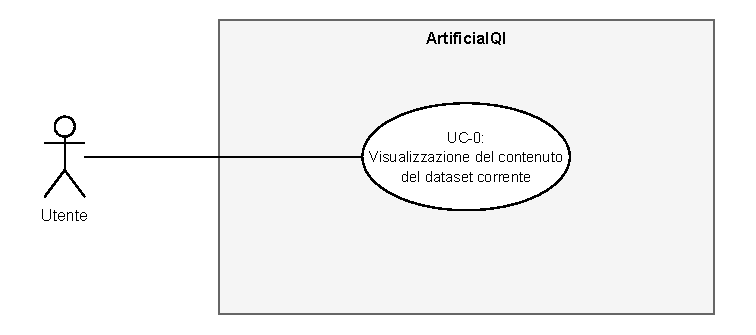
\includegraphics{Sezioni/UseCase/Immagini/UC-0.pdf}
    \caption{Diagramma UC-0.}
\end{figure}

\begin{usecase}{UC-0}{Visualizzazione di un dataset}
    
    \req{\hyperref[item:RU-1]{RU-1}} 

    \pre{
        \item Il sistema è attivo e funzionante
        \item Il dataset esiste
    }

    \post{
        \item Viene visualizzato il dataset
    }
    
    \actor{Utente}

    \subactors{}

    \trigger{L'utente deve visualizzare il dataset}
    
    \inc{}

    \base{}

    \scenario{
        \item L'utente richiede la visualizzazione del dataset
        \item Le coppie del dataset vengono mostrate in una lista
    }

    \subscenario{
        \item[2.1] \textbf{Il dataset è vuoto}
        \begin{itemize}
            \item[a.] Viene indicato all'utente che il dataset è vuoto
        \end{itemize}
    }
\end{usecase}

\subsection{UC-1}
\begin{figure}[H]
    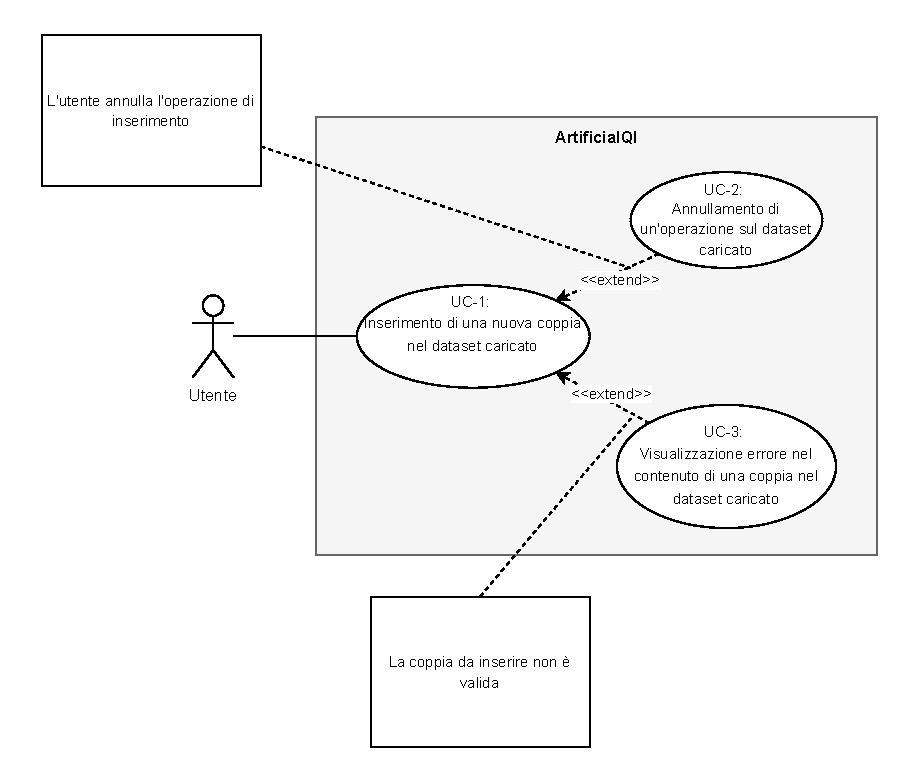
\includegraphics[scale=0.8]{Sezioni/UseCase/Immagini/UC-1.pdf}
    \caption{Diagramma UC-1.}
\end{figure}


\begin{usecase}{UC-1}{Inserimento di una nuova coppia nel dataset corrente}
    
    \req{\hyperref[item:RU-1]{RU-1}} 

    \pre{
        \item Il sistema è attivo e funzionante
    }

    \post{
        \item Viene inserita una nuova coppia nel dataset corrente
    }
    
    \actor{Utente}

    \subactors{}

    \trigger{L'utente vuole inserire di una nuova coppia nel dataset corrente}
    
    \inc{}

    \base{}

    \scenario{
        \item L'utente richiede l'inserimento di una nuova coppia
        \item L'utente specifica il contenuto per la nuova coppia
        \item L'utente conferma l'inserimento della nuova coppia
        \item La coppia viene inserita nel dataset corrente
    }

    \subscenario{
        \item[2.1] \textbf{L'utente annulla l'operazione di inserimento} 
        \begin{itemize}
            \item[a.] \hyperref[subsec:UC-2]{UC-2}
        \end{itemize}
        \item[3.1] \textbf{La coppia da inserire non è valida}
        \begin{itemize}
            \item[a.] \hyperref[subsec:UC-3]{UC-3}
        \end{itemize}
    }
\end{usecase}




\subsection{UC-2}
\label{subsec:UC-2}
\begin{usecase}{UC-2}{Annullamento di un'operazione sul dataset caricato}

        \req{}
        
        \pre{
            \item Il sistema è attivo e funzionante     
            \item L'utente è coinvolto in un'operazione di modifica del dataset caricato
        }
        
        \post{ 
            \item L'operazione viene interrotta 
            \item Il dataset caricato resta invariato
        }

        \actor{Utente}
        
        \subactors{}
        
        \trigger{L'utente richiede l'annullamento dell'operazione}
        
        \inc{}
        
        \base{}
        
        \scenario{
            \item L'utente richiede l'annullamento dell'operazione sul dataset caricato 
            \item La modifica al dataset caricato viene annullata 
            \item Il dataset caricato resta invariato 
        }
        
        
\end{usecase}

\subsection{UC-3}
\label{subsec:UC-3}

\begin{usecase}{UC-3}{Visualizzazione errore nel contenuto di una coppia del dataset corrente}
            
    \req{}
    
    \pre{
        \item Il sistema è attivo e funzionante
        \item Sia la domanda che la risposta della coppia sono vuote
    }
    
    \post {
        \item Viene richiesta la correzione della coppia
    }
    
    \actor{Utente}
    
    \subactors{}

    \trigger{Una coppia è invalida}
    
    \inc{}
    
    \base{}
    
    \scenario{
        \item Viene visualizzato un messaggio di errore che richiede la corretta compilazione di almeno una tra domanda e risposta
    }
\end{usecase}


\subsection{UC-4}

\begin{figure}[H]
    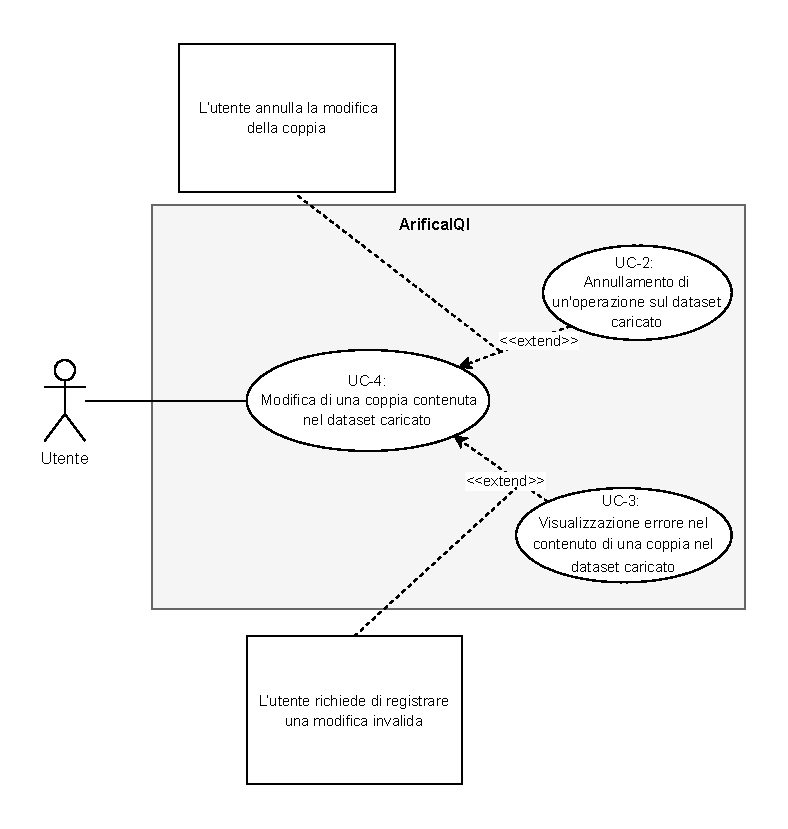
\includegraphics[scale=0.8]{Sezioni/UseCase/Immagini/UC-4.pdf}
    \caption{Diagramma UC-4.}
\end{figure}

\begin{usecase}{UC-4}{Modifica di una coppia contenuta nel dataset corrente}
    
    \req{\hyperref[item:RU-1]{RU-1}} 

    \pre{
        \item Il sistema è attivo e funzionante
        \item Il dataset corrente non è vuoto
        \item La coppia da modificare esiste
    }

    \post{
        \item La coppia viene aggiornata
        \item Il dataset corrente viene aggiornato
    }
    
    \actor{Utente}

    \subactors{}

    \trigger{L'utente deve modificare una coppia contenuta nel dataset corrente}
    
    \inc{}

    \base{}

    \scenario{
        \item L'utente richiede la modifica di una coppia
        \item L'utente modifica il contenuto della coppia
        \item L'utente conferma la modifica della coppia
        \item La coppia viene aggiornata nel dataset corrente

    }

    \subscenario{
        \item[2.1] \textbf{L'utente annulla la modifica della coppia} 
        \begin{itemize}
            \item[a.] \hyperref[subsec:UC-2]{UC-2}
        \end{itemize}
        \item[3.1] \textbf{L'utente richiede di registrare una modifica invalida}
        \begin{itemize}
            \item[a.] \hyperref[subsec:UC-3]{UC-3}
        \end{itemize}
    }
\end{usecase}


\subsection{UC-5}

\begin{figure}[H]
    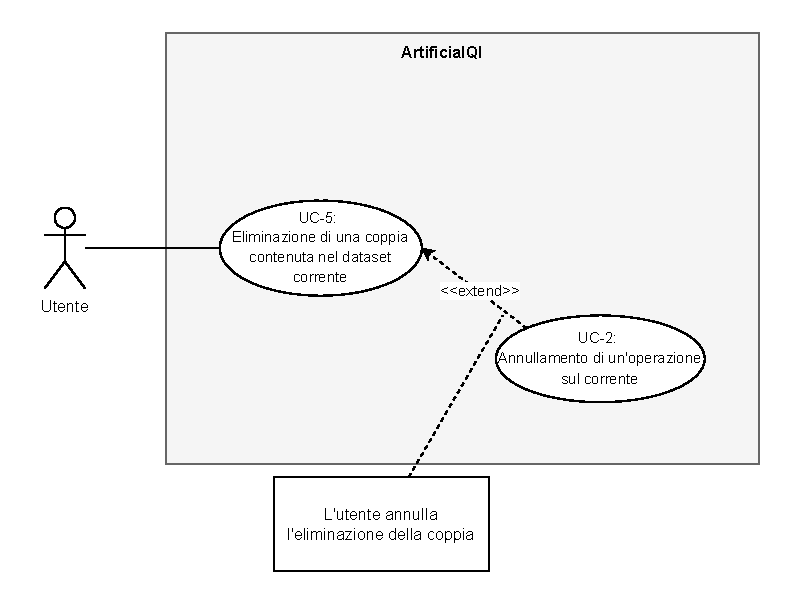
\includegraphics{Sezioni/UseCase/Immagini/UC-5.pdf}
    \caption{Diagramma UC-5.}
\end{figure}

\begin{usecase}{UC-5}{Eliminazione di una coppia contenuta nel dataset corrente}
    
    \req{\hyperref[item:RU-1]{RU-1}} 

    \pre{
        \item Il sistema è attivo e funzionante
        \item Il dataset corrente non è vuoto
        \item La coppia da eliminare esiste
    }

    \post{
        \item La coppia viene eliminata dal dataset corrente
    }
    
    \actor{Utente}

    \subactors{}

    \trigger{L'utente deve eliminare una coppia contenuta nel dataset corrente}
    
    \inc{}

    \base{}

    \scenario{
        \item L'utente richiede l'eliminazione della coppia
        \item L'utente conferma l'eliminazione
        \item La coppia viene eliminata dal dataset corrente
    }

    \subscenario{
        \item[2.1] \textbf{L'utente annulla l'eliminazione della coppia:} 
        \begin{itemize}
            \item[a.] \hyperref[subsec:UC-2]{UC-2}
        \end{itemize}
    }
\end{usecase}


\subsection{UC-6}

\begin{figure}[H]
    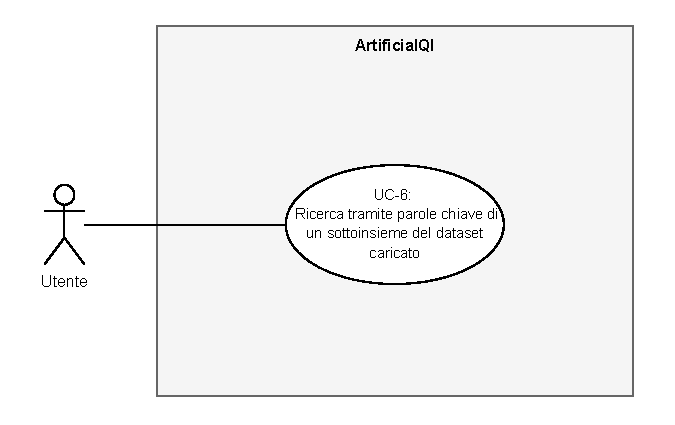
\includegraphics{Sezioni/UseCase/Immagini/UC-6.pdf}
    \caption{Diagramma UC-6.}
\end{figure}

\begin{usecase}{UC-6}{Ricerca tramite parole chiave di un sottoinsieme del dataset corrente}
    
    \req{\hyperref[item:RU-2]{RU-2}} 

    \pre{
        \item Il sistema è attivo e funzionante
        \item Il dataset su cui effettuare la ricerca è stato caricato come dataset corrente
        \item Il dataset corrente non è vuoto
    }

    \post{
        \item Viene mostrato il sottoinsieme del dataset corrente risultante dall'operazione di ricerca
    }
    
    \actor{Utente}

    \subactors{}

    \trigger{L'utente deve cercare una o più coppie contenute nel dataset corrente}
    
    \inc{}

    \base{}

    \scenario{
        \item L'utente specifica le parole chiave
        \item L'utente conferma l'esecuzione della ricerca
        \item Viene mostrata la lista di coppie che contengono le parole chiave nella domanda e/o nella risposta
    }

    \subscenario{
        \item[1.1] \textbf{Non vengono indicate parole chiave}
        \begin{itemize}
            \item [a.] L'utente conferma l'esecuzione della ricerca
            \item [b.] Viene mostrato l'intero dataset corrente
        \end{itemize}
        \item[3.1]\textbf{Il sottoinsieme risultante è vuoto}
        \begin{itemize}
            \item[a.] Viene notificato all'utente che la ricerca non ha prodotto risultati
        \end{itemize}
    }
\end{usecase}


\subsection{UC-7}

\begin{figure}[H]
    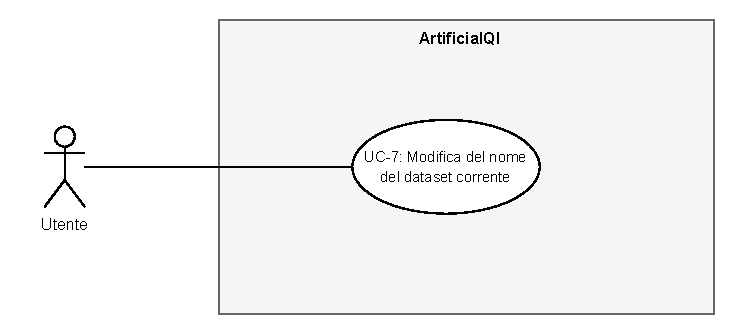
\includegraphics{Sezioni/UseCase/Immagini/UC-7.pdf}
    \caption{Diagramma UC-7.}
\end{figure}

\begin{usecase}{UC-7}{Modifica del nome di un dataset }
    
    \req{\hyperref[item:RU-1]{RU-1}} 

    \pre{
        \item Il sistema è attivo e funzionante
        \item Il dataset da rinominare esiste
    }

    \post{
        \item Il dataset viene rinominato
    }
    
    \actor{Utente}

    \subactors{}

    \trigger{L'utente vuole modificare il nome di un dataset }
    
    \inc{}

    \base{}

    \scenario{
        \item L'utente richiede la modifica del nome di un dataset 
        \item L'utente specifica il nuovo nome
        \item L'utente conferma la modifica 
        \item Il dataset viene rinominato
    }

    \subscenario{
        \item[2.1] \textbf{L'utente annulla l'operazione di modifica}
        \begin{itemize}
            \item [a.] Il nome del dataset resta invariato
            \item [b.] L'operazione di modifica viene terminata
        \end{itemize}
        \item[3.1] \textbf{Il nuovo nome del dataset è vuoto o già esiste}
        \begin{itemize}
            \item [a.] \hyperref[subsec:UC-8]{UC-8}
        \end{itemize}
    }
\end{usecase}

\subsection{UC-8}
\label{subsec:UC-8}

\begin{usecase}{UC-8}{Visualizzazione errore nel nome di un dataset}
    
    \req{} 

    \pre{
        \item Il sistema è attivo e funzionante
        \item Il nome del dataset è invalido
    }

    \post{
        \item Viene richiesto all'utente di fornire un nome valido
    }
    
    \actor{Utente}

    \subactors{}

    \trigger{Il nome del dataset è invalido}
    
    \inc{}

    \base{}

    \scenario{
        \item Viene visualizzato un messaggio di errore che richiede
        la corretta compilazione del nome del dataset
    }
\end{usecase}

\subsection{UC-9}
\label{subsec:UC-9}


\begin{figure}[H]
    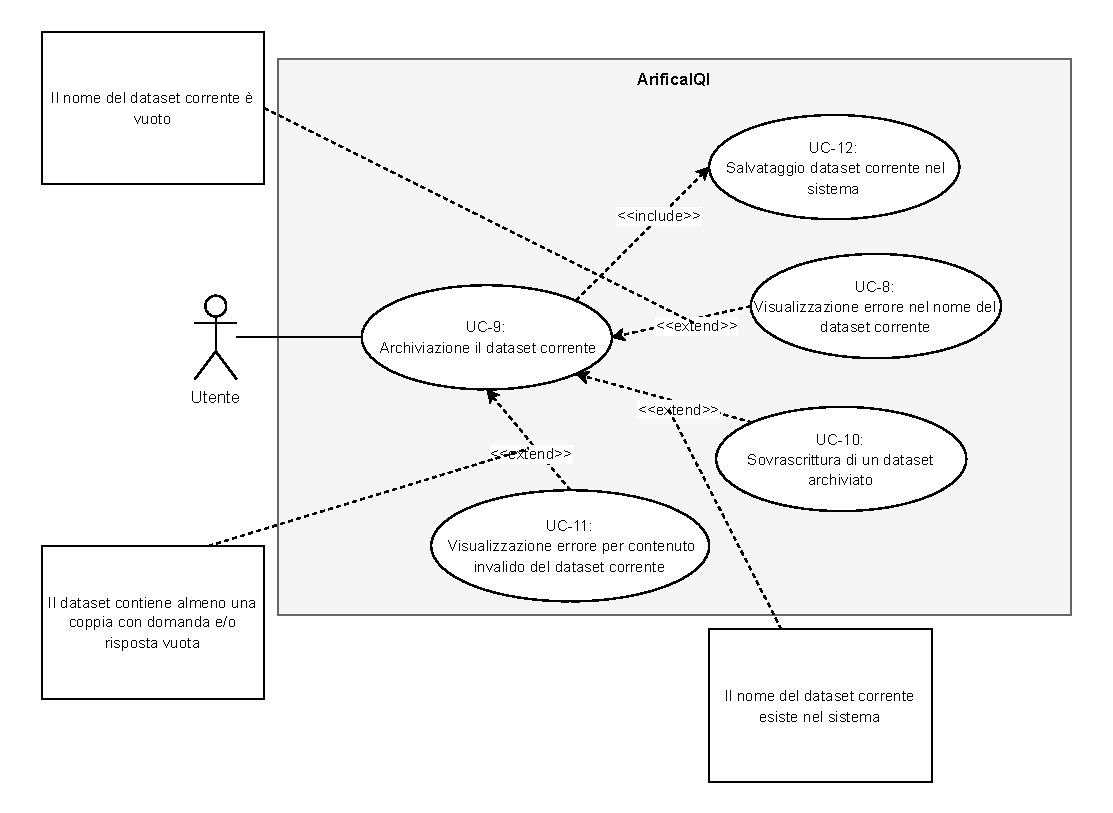
\includegraphics[scale=0.75]{Sezioni/UseCase/Immagini/UC-9.pdf}
    \caption{Diagramma UC-9.}
\end{figure}

\begin{usecase}{UC-9}{Archiviazione del dataset corrente}
    
    \req{\hyperref[item:RU-3]{RU-3}} 

    \pre{
        \item Il sistema è attivo e funzionante
        \item Il dataset corrente non è vuoto
    }

    \post{
        \item Il dataset corrente viene archiviato nel sistema
    }
    
    \actor{Utente}

    \subactors{}

    \trigger{L'utente deve archiviare il dataset corrente per renderlo persistente}
    
    \inc{\hyperref[subsec:UC-12]{UC-12}}

    \base{}

    \scenario{
        \item L'utente richiede l'archiviazione del dataset corrente.
        \item \texttt{<<include:UC-12>>}
    }

    \subscenario{
        \item[1.1] \textbf{Il nome del dataset corrente è vuoto}
        \begin{itemize}
            \item [a.] \hyperref[subsec:UC-8]{UC-8}
        \end{itemize}
        \item[1.2]\textbf{Esiste già un dataset archiviato nel sistema con nome uguale al dataset corrente}
        \begin{itemize}
            \item[a.] \hyperref[subsec:UC-10]{UC-10}
        \end{itemize}
        \item[1.3] \textbf{Il dataset contiene almeno una coppia con domanda e/o risposta vuota}
        \begin{itemize}
            \item[a.] \hyperref[subsec:UC-11]{UC-11}
        \end{itemize}
    }
\end{usecase}


\subsection{UC-10}
\label{subsec:UC-10}

\begin{usecase}{UC-10}{Sovrascrittura di un dataset archiviato}
    \req{\hyperref[item:RU-3]{RU-3}} 

    \pre{
        \item Il sistema è attivo e funzionante
        \item Il dataset corrente possiede già una versione archiviata
    }

    \post{
        \item La versione archiviata del dataset corrente viene sovrascritta
    }
    
    \actor{Utente}

    \subactors{}

    \trigger{L'utente deve aggiornare la versione archiviata di un dataset}
    
    \inc{\hyperref[subsec:UC-12]{UC-12}}

    \base{}

    \scenario{
        \item L'utente richiede l'archiviazione del dataset corrente che possiede già una versione archiviata.
        \item L'utente conferma la sovrascrittura
        \item \texttt{<<include:UC-12>>}
    }

    \subscenario{
        \item[2.1] \textbf{L'utente non conferma la sovrascrittura}
        \begin{itemize}
            \item [a.] L'operazione di sovrascrittura viene interrotta
        \end{itemize}
    }
\end{usecase}

\subsection{UC-11}
\label{subsec:UC-11}

\begin{usecase}{UC-11}{Visualizzazione errore per contenuto invalido del dataset corrente}
    \req{} 

    \pre{
        \item Il sistema è attivo e funzionante
        \item Il dataset corrente contiene almeno una coppia invalida ovvero avente domanda e/o risposta vuota
    }

    \post{
        \item L'utente conosce le coppie invalide contenute nel dataset corrente
    }
    
    \actor{Utente}

    \subactors{}

    \trigger{Il dataset corrente contiene almeno una coppia invalida}
    
    \inc{}

    \base{}

    \scenario{
        \item Viene notificata all'utente la presenza di coppie invalide
        \item Vengono evidenziate le coppie invalide
    }
\end{usecase}

\subsection{UC-12}
\label{subsec:UC-12}

\begin{figure}[H]
    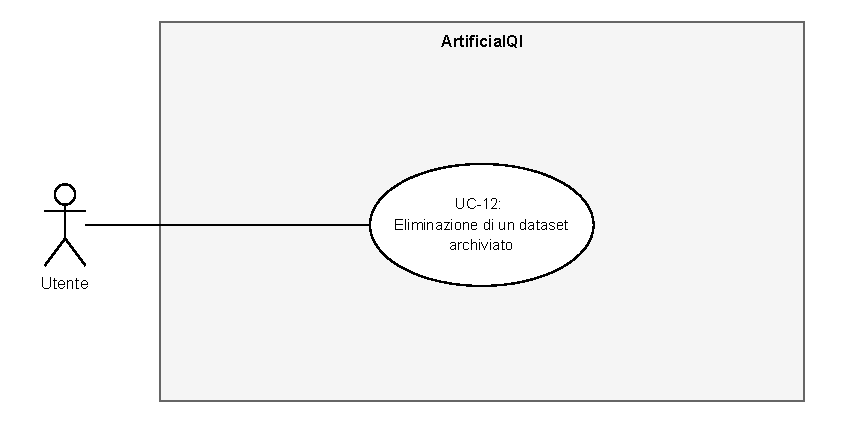
\includegraphics{Sezioni/UseCase/Immagini/UC-12.pdf}
    \caption{Diagramma UC-12.}
\end{figure}

\begin{usecase}{UC-12}{Eliminazione di un dataset archiviato}

    \req{\hyperref[item:RU-3]{RU-3}} 

    \pre{
        \item Il sistema è attivo e funzionante
        \item Il dataset archiviato da eliminare esiste
    }

    \post{
        \item Il dataset selezionato viene eliminato 
    }
    
    \actor{Utente}

    \subactors{}

    \trigger{L'utente deve eliminare un dataset archiviato}
    
    \inc{}

    \base{}

    \scenario{
        \item L'utente richiede l'eliminazione di un dataset archiviato
        \item L'utente conferma l'eliminazione del dataset selezionato
        \item Il dataset viene eliminato dal sistema
    }

    \subscenario{
        \item[2.1] \textbf{L'utente annulla l'eliminazione del dataset selezionato}
        \begin{itemize}
            \item[a.] Il dataset selezionato non viene eliminato
            \item[b.] Viene interrotta l'operazione di eliminazione
        \end{itemize}
        \item[3.1] \textbf{L'eliminazione del dataset dal sistema produce un errore}
        \begin{itemize}
        \item[a.] Viene notificato all'utente l'errore che ha impedito la corretta eliminazione del dataset selezionato
        \end{itemize}
    }

\end{usecase}

\subsection{UC-13}
\label{subsec:UC-13}

\begin{figure}[H]
    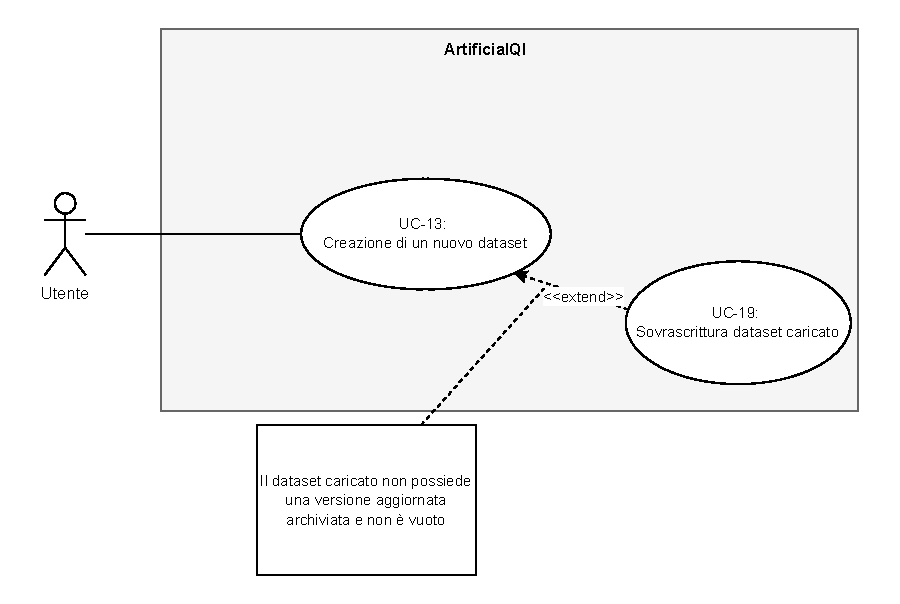
\includegraphics{Sezioni/UseCase/Immagini/UC-13.pdf}
    \caption{Diagramma UC-13.}
\end{figure}

\begin{usecase}{UC-13}{Creazione di un nuovo dataset}

    \req{\hyperref[item:RU-3]{RU-3}} 

    \pre{
        \item Il sistema è attivo e funzionante
    }

    \post{
        \item Il nuovo dataset temporaneo viene caricato
    }
    
    \actor{Utente}

    \subactors{}

    \trigger{L'utente deve creare un nuovo dataset}
    
    \inc{}

    \base{}

    \scenario{
        \item L'utente richiede la creazione di un nuovo dataset
        \item Viene creato un nuovo dataset temporaneo vuoto
        \item Il dataset temporaneo viene caricato
    }

    \subscenario{
        \item[2.1] \textbf{Il dataset caricato non possiede una versione aggiornata archiviata e non è vuoto}
        \begin{itemize}
            \item[a.] \hyperref[subsec:UC-19]{UC-19}
        \end{itemize}
    }

\end{usecase}

\subsection{UC-14}
\label{subsec:UC-14}

\begin{figure}[H]
    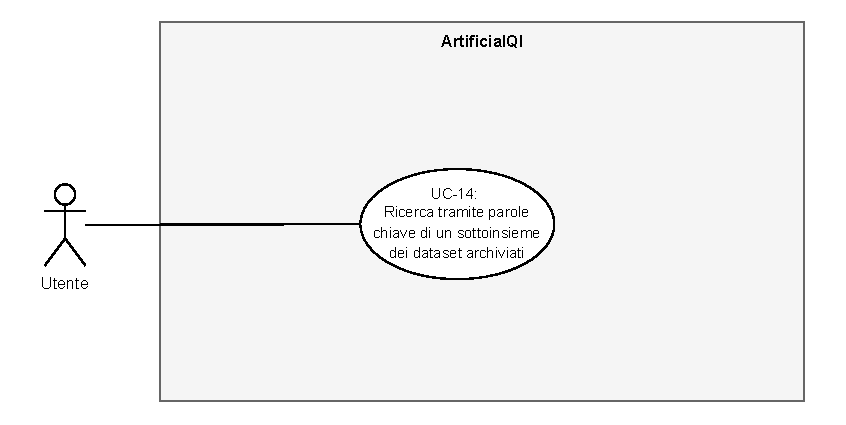
\includegraphics{Sezioni/UseCase/Immagini/UC-14.pdf}
    \caption{Diagramma UC-14.}
\end{figure}

\begin{usecase}{UC-14}{Caricamento di un dataset archiviato}

    \req{\hyperref[item:RU-4]{RU-4}} 

    \pre{
        \item Il sistema è attivo e funzionante
        \item Il dataset da caricare è stato precedentemente archiviato
    }

    \post{
        \item Il dataset viene caricato
    }
    
    \actor{Utente}

    \subactors{}

    \trigger{L'utente deve caricare un dataset tra quelli archiviati nel sistema}
    
    \inc{}

    \base{}

    \scenario{
        \item L'utente richiede di caricare un dataset archiviato nel sistema
        \item L'utente seleziona il nome del dataset tra quelli archiviati
        \item Il dataset scelto viene caricato
    }

    \subscenario{
        \item[3.1] \textbf{Il dataset caricato non possiede una versione aggiornata archiviata e non è vuoto}
        \begin{itemize}
            \item[a.] \hyperref[subsec:UC-15]{UC-15}
        \end{itemize}
    }
\end{usecase}

\subsection{UC-15}
\label{subsec:UC-15}


\begin{figure}[H]
    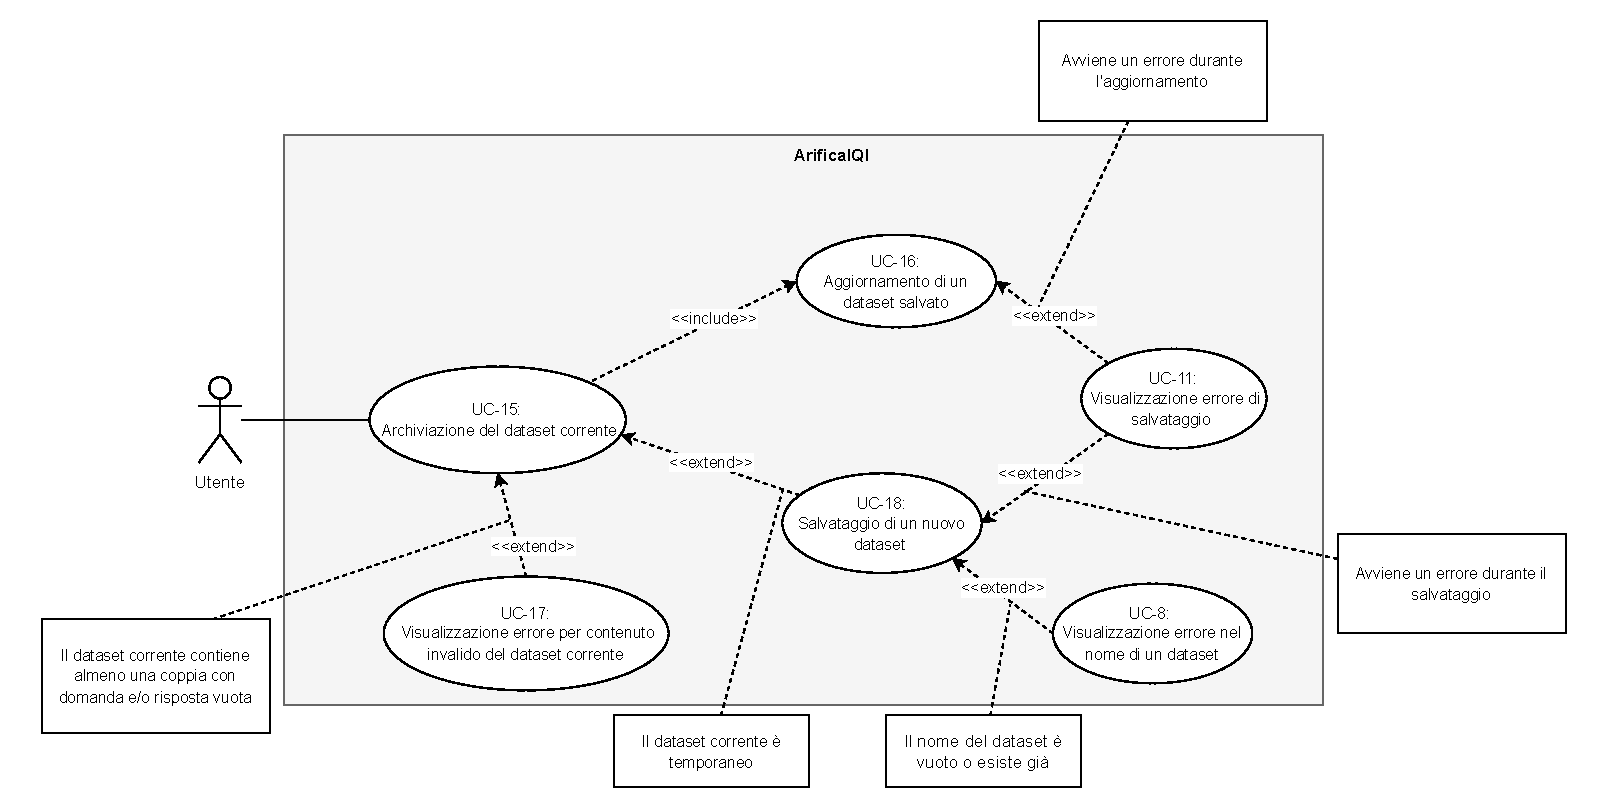
\includegraphics[scale=0.60]{Sezioni/UseCase/Immagini/UC-15.pdf}
    \caption{Diagramma UC-15.}
\end{figure}

\begin{usecase}{UC-15}{Archiviazione del dataset corrente}
    
    \req{\hyperref[item:RU-5]{RU-5}} 

    \pre{
        \item Il sistema è attivo e funzionante
        \item Il dataset da archiviare è stato caricato come dataset corrente
        \item Il dataset corrente non è vuoto
        \item Il dataset corrente non possiede una copia archiviata aggiornata
    }

    \post{
        \item Il dataset corrente viene archiviato nel sistema
    }
    
    \actor{Utente}

    \subactors{}

    \trigger{L'utente deve archiviare il dataset corrente per renderlo persistente}
    
    \inc{\hyperref[subsec:UC-16]{UC-16}}

    \base{}

    \scenario{
        \item L'utente richiede l'archiviazione del dataset corrente.
        \item \texttt{<<include:UC-16>>}
    }

    \subscenario{
        \item[1.1] \textbf{Il dataset corrente contiene almeno una coppia con domanda e/o risposta vuota}
        \begin{itemize}
            \item[a.] \hyperref[subsec:UC-17]{UC-17}
        \end{itemize}
        \item[1.2] \textbf{Il dataset corrente è temporaneo perchè è stato appena creato}
        \begin{itemize}
            \item[a.] \hyperref[subsec:UC-18]{UC-18}
        \end{itemize}
    }
\end{usecase}


\subsection{UC-16}
\label{subsec:UC-16}

\begin{usecase}{UC-16}{Salvataggio del dataset caricato nel sistema}
    \req{} 

    \pre{
        \item Il sistema è attivo e funzionante
    }

    \post{
        \item Il dataset caricato viene salvato nel sistema
        \item L'utente è a conoscenza del corretto salvataggio
    }
    
    \actor{Utente}

    \subactors{}

    \trigger{Il sistema deve salvare il dataset caricato}
    
    \inc{}

    \base{}

    \scenario{
        \item Il dataset caricato viene salvato nel sistema
    }

    \subscenario{
        \item[1.1] \textbf{Avviene un errore durante il salvataggio del dataset caricato}
        \begin{itemize}
            \item[a.] \hyperref[subsec:UC-11]{UC-11}
        \end{itemize}
    }

\end{usecase}

\subsection{UC-17}
\label{subsec:UC-17}

\begin{figure}[H]
    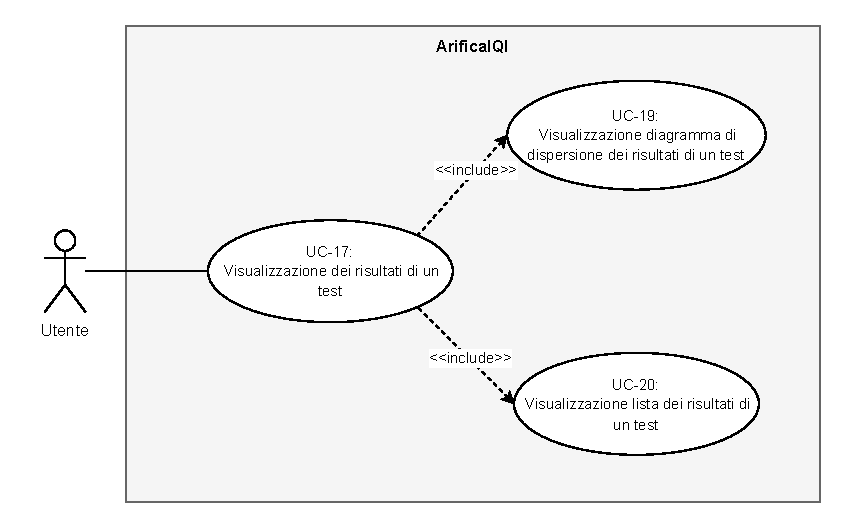
\includegraphics{Sezioni/UseCase/Immagini/UC-17.pdf}
    \caption{Diagramma UC-17.}
\end{figure}

\begin{usecase}{UC-17}{Visualizzazione dei risultati di un test}

    \req{\hyperref[item:RU-6]{RU-6}} 

    \pre{
        \item Il sistema è attivo e funzionante
        \item Sono disponibili i risultati di un test
    }

    \post{
        \item L'utente conosce l'esito del test
    }
    
    \actor{Utente}

    \subactors{}

    \trigger{L'utente deve testare il LLM usando il dataset corrente}
    
    \inc{\hyperref[subsec:UC-19]{UC-19}, \hyperref[subsec:UC-20]{UC-20}}

    \base{}

    \scenario{
        \item \texttt{<<include:UC-19>>}
        \item \texttt{<<include:UC-20>>}
    }

\end{usecase}

\subsection{UC-18}
\label{subsec:UC-18}

\begin{figure}[H]
    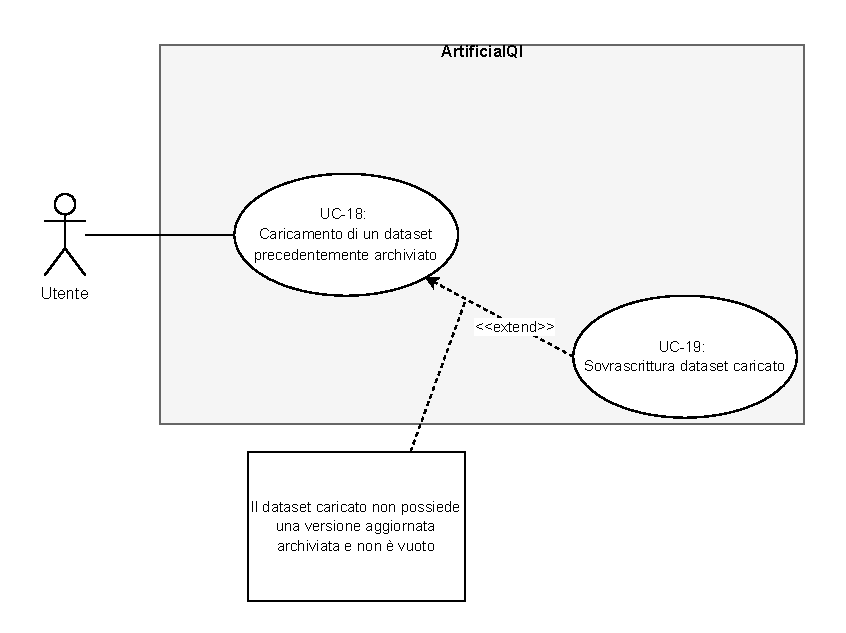
\includegraphics{Sezioni/UseCase/Immagini/UC-18.pdf}
    \caption{Diagramma UC-18.}
\end{figure}

\begin{usecase}{UC-18}{Caricamento di un dataset archiviato}

    \req{\hyperref[item:RU-6]{RU-6}} 

    \pre{
        \item Il sistema è attivo e funzionante
        \item Il dataset da caricare è stato precedentemente archiviato
    }

    \post{
        \item Il dataset viene caricato
    }
    
    \actor{Utente}

    \subactors{}

    \trigger{L'utente deve caricare un dataset tra quelli archiviati nel sistema}
    
    \inc{}

    \base{}

    \scenario{
        \item L'utente richiede di caricare un dataset archiviato nel sistema
        \item L'utente seleziona il nome del dataset tra quelli archiviati
        \item Il dataset scelto viene caricato
    }

    \subscenario{
        \item[3.1] \textbf{Il dataset caricato non possiede una versione aggiornata archiviata e non è vuoto}
        \begin{itemize}
            \item[a.] \hyperref[subsec:UC-19]{UC-19}
        \end{itemize}
    }
\end{usecase}

\subsection{UC-19}
\label{subsec:UC-19}

\begin{figure}[H]
    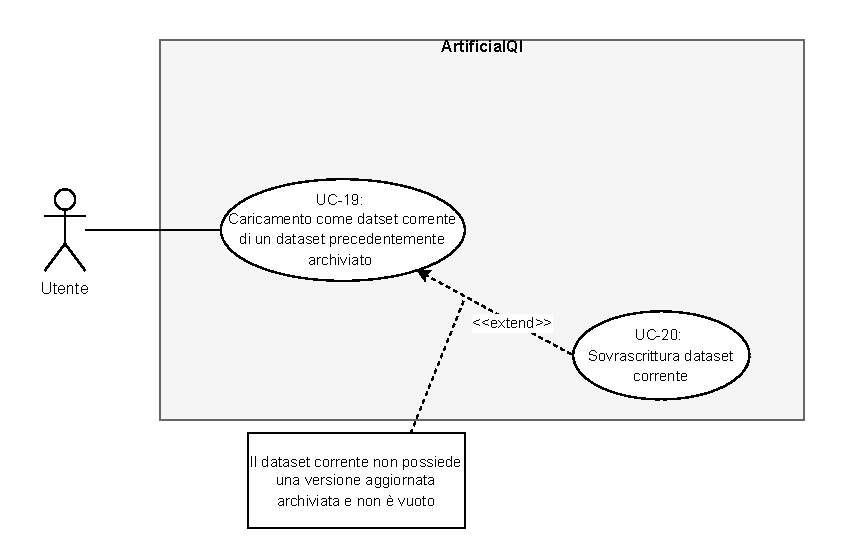
\includegraphics{Sezioni/UseCase/Immagini/UC-19.pdf}
    \caption{Diagramma UC-19.}
\end{figure}

\begin{usecase}{UC-19}{Caricamento come dataset corrente di un dataset archiviato}

    \req{\hyperref[item:RU-6]{RU-6}} 

    \pre{
        \item Il sistema è attivo e funzionante
        \item Il dataset da caricare come dataset corrente è stato precedentemente archiviato
    }

    \post{
        \item Il dataset viene caricato come dataset corrente
    }
    
    \actor{Utente}

    \subactors{}

    \trigger{L'utente deve caricare come dataset corrente uno tra quelli archiviati}
    
    \inc{}

    \base{}

    \scenario{
        \item L'utente richiede di caricare un dataset archiviato
        \item L'utente seleziona il nome del dataset tra quelli archiviati
        \item Il dataset scelto viene caricato come dataset corrente
    }

    \subscenario{
        \item[3.1] \textbf{Il dataset caricato non possiede una versione aggiornata archiviata e non è vuoto}
        \begin{itemize}
            \item[a.] \hyperref[subsec:UC-20]{UC-20}
        \end{itemize}
    }
\end{usecase}

\subsection{UC-20}
\label{subsec:UC-20}

\begin{usecase}{UC-20}{Visualizzazione lista dei risultati di un test}

    \req{\hyperref[item:RU-6]{RU-6}} 

    \pre{
        \item Il sistema è attivo e funzionante
        \item È stato eseguito correttamente il test sul dataset caricato
    }

    \post{
        \item L'utente visualizza la lista dei risultati del test
    }
    
    \actor{Utente}

    \subactors{LLM}

    \trigger{}
    
    \inc{}

    \base{}

    \scenario{
        \item Viene mostrata la lista dei risultati del test.
        
        
        \item Ogni elemento è composto da: domanda, risposta attesa, risposta ottenuta dal LLM, grado di somiglianza tra le due risposte e valutazione di correttezza della risposta.
    }

\end{usecase}

\subsection{UC-21}
\label{subsec:UC-21}

\begin{usecase}{UC-21}{Visualizzazione errore di comunicazione con LLM}

    \req{} 

    \pre{
        \item Il sistema è attivo e funzionante
        \item La comunicazione con il LLM non è andata a buon fine
    }

    \post{
        \item L'utente conosce l'errore di comunicazione
    }
    
    \actor{Utente}

    \subactors{LLM}

    \trigger{La comunicazione con il LLM produce un errore}
    
    \inc{}

    \base{}

    \scenario{
        \item Viene mostrato un messaggio di errore all'utente
    }

\end{usecase}

\subsection{UC-22}
\label{subsec:UC-22}

\begin{usecase}{UC-22}{Eliminazione di un dataset archiviato}

    \req{\hyperref[item:RU-6]{RU-6}} 

    \pre{
        \item Il sistema è attivo e funzionante
        \item Il dataset archiviato da eliminare esiste
    }

    \post{
        \item Il dataset selezionato viene eliminato 
    }
    
    \actor{Utente}

    \subactors{}

    \trigger{L'utente deve eliminare un dataset archiviato}
    
    \inc{}

    \base{}

    \scenario{
        \item L'utente richiede l'eliminazione di un dataset archiviato
        \item L'utente conferma l'eliminazione del dataset selezionato
        \item Il dataset viene eliminato dal sistema
    }

    \subscenario{
        \item[2.1] \textbf{L'utente annulla l'eliminazione del dataset selezionato}
        \begin{itemize}
            \item[a.] Il dataset selezionato non viene eliminato
            \item[b.] Viene interrotta l'operazione di eliminazione
        \end{itemize}
        \item[3.1] \textbf{L'eliminazione del dataset dal sistema produce un errore}
        \begin{itemize}
        \item[a.] Viene notificato all'utente l'errore che ha impedito la corretta eliminazione del dataset selezionato
        \end{itemize}
    }

\end{usecase}

\subsection{UC-23}
\label{subsec:UC-23}

\begin{usecase}{UC-23}{Visualizzazione errore di salvataggio del dataset}
    \req{} 

    \pre{
        \item Il sistema è attivo e funzionante
    }

    \post{
        \item L'utente conosce la causa del errore di salvataggio
    }
    
    \actor{Utente}

    \subactors{}

    \trigger{Il sistema riscontra un errore nel salvataggio del dataset }
    
    \inc{}

    \base{}

    \scenario{
        \item Viene notificato all'utente l'errore che ha impedito il corretto salvataggio del dataset 
    }

\end{usecase}

\subsection{UC-24}
\label{subsec:UC-24}

\begin{usecase}{UC-24}{Visualizzazione diagramma di dispersione dei risultati di un test}

    \req{} 

    \pre{
        \item Il sistema è attivo e funzionante
        \item È stato eseguito correttamente il test sul dataset caricato
    }

    \post{
        \item L'utente visualizza un diagramma di dispersione
    }
    
    \actor{Utente}

    \subactors{LLM}

    \trigger{}
    
    \inc{}

    \base{}

    \scenario{
        \item Visualizzazione di un grafico di dispersione.
        L'asse delle ordinate rappresenta il numero della domanda.
        L'asse delle ascisse rappresenta il grado di somiglianza tra la risposta attesa e la risposta effettiva.
        
        \item Rappresentazione dei risultati come punti distinguibili tra risposta corretta e sbagliata.
        
        \item Calcolo della media e rappresentazione come una retta nel grafico.
        
        \item Calcolo della deviazione standard come una retta nel grafico.
        
        \item Mostrare la legenda del grafico.
    }

\end{usecase}

\subsection{UC-25}
\label{subsec:UC-25}

\begin{figure}[H]
    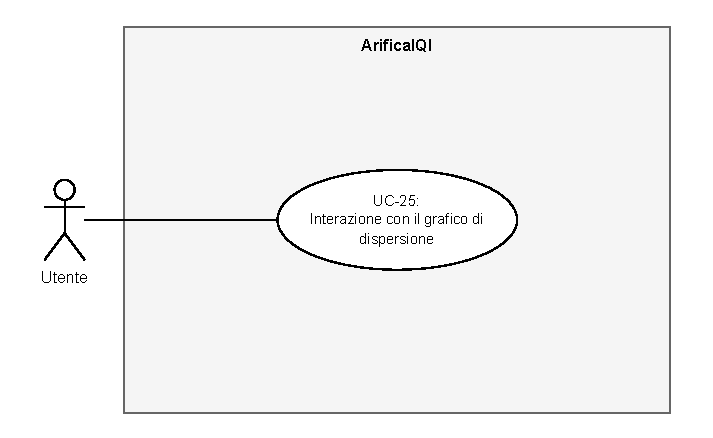
\includegraphics{Sezioni/UseCase/Immagini/UC-25.pdf}
    \caption{Diagramma UC-25.}
\end{figure}

\begin{usecase}{UC-25}{Interazione con il grafico di dispersione}

    \req{} 

    \pre{
        \item Il sistema è attivo e funzionante
        \item L'utente dispone del grafico di dispersione prodotto nella visualizzazione dei risultati del test
    }

    \post{
        \item Viene evidenziato il risultato relativo al punto del grafico di dispersione coinvolto nell'interazione.
    }
    
    \actor{Utente}

    \subactors{LLM}

    \trigger{L'utente ha la necessità di visualizzare un preciso risultato}
    
    \inc{}

    \base{}

    \scenario{
        \item L'utente interagisce con un punto del grafico di dispersione.
        
        
        \item Viene evidenziato l'elemento della lista dei risultati corrispondente al punto coinvolto nell'interazione.
    }

\end{usecase}

\section{Requisiti Software}
\label{sec:requisiti_software}
In questa sezione vengono elencati i \glossario{requisiti software} individuati dal gruppo per la realizzazione del progetto ArtificialQI.
I requisiti sono stati definiti tramite l'analisi dei \glossario{requisiti utente} tramite i diagrammi \glossario{use case}.
I \glossario{requisiti software} si dividono in:
\begin{enumerate}
    \label{en:req_type}
    \item Requisiti funzionali: definiscono le funzionalità attese dal sistema.
    \item Requisiti non funzionali: definiscono gli attributi attesi del sistema nel suo insieme.
    Si dividono in:
    \begin{enumerate}
        \item Requisiti di qualità: impongono dei vincoli sulla qualità del prodotto.
        \item Requisiti di vincolo: impongono dei vincoli sullo svolgimento del progetto.
    \end{enumerate}
\end{enumerate}
Ogni \glossario{requisito software} viene descritto indicando le seguenti informazioni:
\begin{enumerate}
    \item Identificativo che segue la sintassi:
    \begin{lstlisting}
        R<T><O/F>-<N>
    \end{lstlisting}
    Dove:
    \begin{enumerate}
        \item \lstinline{T} indica il tipo di requisito software che può variare tra \lstinline{F}(funzionali), \lstinline{Q}(di qualità) e \lstinline{V}(di vincolo).
        \item \lstinline{O} indica che il requisito è obbligatorio mentre \lstinline{F} indica che il requisito è facoltativo.
        \item \lstinline{N} è un numero crescente rispetto al tipo di requisito che parte dal valore 1.
    \end{enumerate}
    \item Descrizione testuale.
    \item Specifica ovvero la lista di sotto requisiti che approfondiscono il \glossario{requisito software} principale.
    Ogni sotto requisito è identificato usando l'identificativo del requisito padre a cui viene aggiunto in coda un secondo numero crescente che parte da 1 preceduto da un
    \item Dipendenze con altri \glossario{requisito software} facoltativi.
    \item Una lista dei requisiti utente che hanno dato origine al \glossario{requisito software}.
\end{enumerate}

\subsection{Requisiti funzionali}
\label{subsec:requisiti_funzionali}
I requisiti funzionali sono raggruppati usando una divisione ad alto livello del sistema in due componenti, ovvero 
\begin{enumerate}
    \item Logica di presentazione: si occupa della presentazione delle informazioni agli utenti.
    \item Logica di business: si occupa dell'elaborazione delle informazioni mostrate agli utenti e ottenute dagli utenti.
\end{enumerate}

\subsubsection{Logica di presentazione}

\paragraph{Obbligatori}

\begin{freq}
    [
        \dependency{Se il sistema può gestire un insieme di LLM salvati quando l'utente richiede l'esecuzione di un test deve richiedere l'LLM da testare \hyperref[rf:RFF-1]{RFF-1}}
    ]
    {RFO-1}
    {Il sistema deve permettere la visualizzazione del dataset caricato dall'utente}
    \label{rf:RFO-1}%

    \subreq{RFO-1.01}{UC-1}{Il sistema deve visualizzare il nome del dataset caricato se non è temporaneo altrimenti indicare il fatto che è temporaneo}
    
    \subreq{RFO-1.02}{}{Se il dataset caricato è vuoto, il sistema deve visualizzare un messaggio che lo indica}

    \subreq{RFO-1.03}{}{Se l'utente ha già visualizzato il dataset a partire dal suo caricamento, il sistema deve visualizzare l'ultima pagina richiesta \hyperref[rf:RFO-2]{RFO-2}}
    
    \subreq{RFO-1.04}{}{Se l'utente visualizza per la prima volta il dataset a partire dal suo caricamento, il sistema deve visualizzare la prima pagina \hyperref[rf:RFO-2]{RFO-2}}
    
    \subreq{RFO-1.05}{}{Il sistema deve visualizzare un elemento che permetta la navigazione tra le pagine del dataset}
    
    \subreq{RFO-1.06}{}{Se il dataset caricato non è vuoto, il sistema deve visualizzare una barra di ricerca che fornisca all'utente le informazioni necessarie per il suo utilizzo}
    
    \subreq{RFO-1.07}{}{Il sistema deve visualizzare un pulsante che permetta l'aggiunta di un elemento al dataset caricato \hyperref[rf:RFO-4]{RFO-4}} 
    
    \subreq{RFO-1.08}{}{Se il dataset non è vuoto, il sistema deve visualizzare un pulsante che permetta l'esecuzione di un test} 
    
    \subreq{RFO-1.09}{}{Se l'utente cerca di eseguire un test su un dataset incompleto il sistema deve visualizzare una lista contenente i link agli elementi incompleti presenti nel dataset caricato \hyperref[rf:RFO-5]{RFO-5}}

    \subreq{RFO-1.10}{}{Se il sistema riscontra un errore durante l'esecuzione del test, deve visualizzare un messaggio di errore}
    
    \subreq{RFO-1.11}{}{Se il dataset caricato contiene modifiche non ancora salvate, il sistema deve visualizzare un pulsante che ne consenta il salvataggio}

    \subreq{RFO-1.12}{}{Se l'utente richiede il salvataggio di un dataset temporaneo, il sistema richiede il nome da assegnargli \hyperref[rf:RFO-6]{RFO-6}}

    \subreq{RFO-1.13}{}{Se il sistema riscontra un errore durante il salvataggio del dataset caricato, deve visualizzare un messaggio di errore}
\end{freq}

\begin{freq}
    {RFO-2}{Il sistema deve poter visualizzare una pagina del dataset caricato}
    \label{rf:RFO-2}%
    
    \subreq{RFO-2.01}{}{Il sistema deve visualizzare la pagina del dataset sotto forma di una lista scorrevole di elementi \hyperref[rf:RFO-3]{RFO-3}}

    \subreq{RFO-2.02}{}{Se il sistema verifica che è stata richiesta una pagina non valida visualizza un messaggio di errore}
        
    \subreq{RFO-2.03}{}{Se il sistema riscontra un errore durante il recupero degli elementi appartenenti alla pagina, deve visualizzare un messaggio di errore}

\end{freq}

\begin{freq}
    {RFO-3}
    {Il sistema deve poter visualizzare un elemento del dataset caricato}
    \label{rf:RFO-3}%
    
    \subreq{RFO-3.01}{}{Il sistema deve visualizzare la domanda contenuta nell'elemento}
    
    \subreq{RFO-3.02}{}{Il sistema deve visualizzare la risposta contenuta nell'elemento}
    
    \subreq{RFO-3.03}{}{Se domanda o risposta sono vuote il sistema deve indicarlo all'utente}
    
    \subreq{RFO-3.04}{}{Il sistema deve visualizzare un bottone che permette la modifica di un elemento \hyperref[rf:RFO-4]{RFO-4}}
    
    \subreq{RFO-3.05}{}{Il sistema deve visualizzare un bottone che permette l'eliminazione di un elemento}

    \subreq{RFO-3.06}{}{Se l'utente richiede l'eliminazione di un elemento il sistema deve richiedere la conferma}

\end{freq}

\begin{freq}
    {RFO-4}
    {Il sistema deve poter visualizzare gli elementi necessari per l'inserimento o la modifica di un elemento nel dataset caricato}
    \label{rf:RFO-4}%
    
    \subreq{RFO-4.01}{}{Il sistema deve visualizzare un elemento di input che permetta di specificare la domanda}
    
    \subreq{RFO-4.02}{}{Il sistema deve visualizzare un elemento di input che permetta di specificare la risposta attesa}
    
    \subreq{RFO-4.03}{}{Il sistema deve visualizzare un bottone che permetta la conferma}
    
    \subreq{RFO-4.04}{}{Il sistema deve visualizzare un bottone che permetta l'annullamento}
    
    \subreq{RFO-4.05}{}{Se si cerca di confermare un elemento non valido, il sistema deve visualizzare un messaggio di errore in cui viene indicato come compilare correttamente l'elemento}

\end{freq}

\begin{freq}
    {RFO-5}
    {Il sistema deve poter visualizzare la lista dei link agli elementi incompleti contenuti nel dataset caricato}
    \label{rf:RFO-5}%
    
    \subreq{RFO-5.01}{}{Il sistema deve visualizzare i link agli elementi incompleti presenti nel dataset usando una lista}
    
    \subreq{RFO-5.02}{}{Ogni link deve avere come ancora di destinazione la pagina del dataset caricato che contiene l'elemento incompleto}

    \subreq{RFO-5.03}{}{Se il sistema riscontra un errore interno durante l'ottenimento delle informazioni sugli elementi incompleti deve visualizzare un messaggio di errore}

\end{freq}

\begin{freq}
    {RFO-6}
    {Il sistema deve poter visualizzare gli elementi necessari per nominare e/o rinominare un dataset}
    \label{rf:RFO-6}%
    
    \subreq{RFO-6.01}{}{Il sistema deve visualizzare un elemento di input che permetta di specificare il nome}
    
    \subreq{RFO-6.02}{}{Il sistema deve visualizzare un bottone che permetta la conferma}
    
    \subreq{RFO-6.03}{}{Il sistema deve visualizzare un bottone che permetta l'annullamento}
    
    \subreq{RFO-6.04}{}{Se si cerca di confermare un elemento non valido il sistema deve visualizzare un messaggio di errore}

\end{freq}

\begin{freq}
    [
        \dependency{Se il sistema può gestire la creazione di un nuovo dataset a partire da un file JSON deve mostrare un pulsante che permetta il caricamento del file \hyperref[rf:RFF-13]{RFF-13}}
    ]
    {RFO-7}
    {Il sistema deve permettere la visualizzazione dei dataset salvati}
    \label{rf:RFO-7}%
    
    \subreq{RFO-7.01}{}{Se non esistono dataset salvati il sistema deve visualizzare un messaggio che lo indica}
    
    \subreq{RFO-7.02}{}{Il sistema deve visualizzare un bottone che permetta la  creazione e il caricamento di un nuovo dataset temporaneo vuoto}
    
    \subreq{RFO-7.03}{}{Il sistema deve visualizzare i dataset salvati sotto forma di una lista scorrevole \hyperref[rf:RFO-8]{RFO-8}}
        
    \subreq{RFO-7.04}{}{Il sistema, se esistono dataset salvati, deve visualizzare una barra di ricerca che specifichi all'utente le informazioni necessarie per l'esecuzione della ricerca stessa}

\end{freq}

\begin{freq}
    {RFO-8}
    {Il sistema deve poter visualizzare un dataset salvato}
    \label{rf:RFO-8}%
    
    \subreq{RFO-8.01}{}{Il sistema deve visualizzare il nome del dataset salvato}
    
    \subreq{RFO-8.02}{}{Il sistema deve visualizzare la data dell'ultima modifica}
    
    \subreq{RFO-8.03}{}{Il sistema deve visualizzare un bottone che permetta di rinominare il dataset salvato \hyperref[rf:RFO-6]{RFO-6}}
    
    \subreq{RFO-8.04}{}{Il sistema deve visualizzare un bottone che permetta di copiare il dataset salvato}
    
    \subreq{RFO-8.05}{}{Il sistema deve visualizzare un bottone che permetta di eliminare il dataset salvato}

    \subreq{RFO-8.06}{}{Se l'utente richiede l'eliminazione di un dataset salvato, il sistema deve richiedere la conferma}
    
    \subreq{RFO-8.07}{}{Il sistema deve visualizzare un bottone che permetta di caricare e visualizzare il dataset salvato \hyperref[rf:RFO-1]{RFO-1}}

    \subreq{RFO-8.08}{}{Se viene richiesto il caricamento di un dataset salvato quando il dataset attualmente caricato contiene modifiche non salvate, il sistema deve richiedere conferma della sovrascrittura}

    \subreq{RFO-8.09}{}{Se il sistema riscontra un errore interno durante l'ottenimento delle informazioni del dataset salvato, il sistema deve visualizzare un messaggio di errore}

 \end{freq}

\begin{freq}
    [
        \dependency{Se il sistema può gestire un insieme di test salvati, deve indicare il nome del test caricato, se non è temporaneo, altrimenti deve indicare il fatto che è temporaneo}
        \dependency{Se il sistema può gestire un insieme di LLM salvati deve visualizzare il nome dell'LLM testato}
        \dependency{Se il sistema può gestire il confronto tra test, deve visualizzare un pulsante che permetta il confronto del test caricato con un test salvato \hyperref[rf:RFF-9]{RFF-9}}
    ]
    {RFO-9}
    {Il sistema deve permettere la visualizzazione del test caricato}
    \label{rf:RFO-9}%
    
    \subreq{RFO-9.01}{}{Il sistema deve indicare la data di esecuzione del test}

    \subreq{RFO-9.02}{}{Il sistema deve visualizzare l'indice riassuntivo \hyperref[rf:RFO-10]{RFO-10}}
    
    \subreq{RFO-9.03}{}{Se l'utente ha già visualizzato il test a partire dal suo caricamento, il sistema deve visualizzare l'ultima pagina richiesta \hyperref[rf:RFO-11]{RFO-11}}
    
    \subreq{RFO-9.04}{}{Se l'utente visualizza per la prima volta il test a partire dal suo caricamento il sistema deve visualizzare la prima pagina \hyperref[rf:RFO-11]{RFO-11}}
    
    \subreq{RFO-9.05}{}{Il sistema deve visualizzare un elemento che permetta la navigazione tra le pagine di risultati}

    \subreq{RFO-9.06}{}{Il sistema deve visualizzare il nome del dataset utilizzato nel test se non è temporaneo}
    
 \end{freq}

 \begin{freq}
    {RFO-10}
    {Il sistema deve poter visualizzare l'indice riassuntivo di un test}
    \label{rf:RFO-10}%
    
    \subreq{RFO-10.01}{}{Il sistema deve visualizzare il numero di domande che compongono il dataset usato nel test}
    
    \subreq{RFO-10.02}{}{Il sistema deve visualizzare la media dei gradi di similarità}

    \subreq{RFO-10.03}{}{Il sistema deve visualizzare la deviazione standard dei gradi di similarità}
    
    \subreq{RFO-10.04}{}{Il sistema deve visualizzare un grafico a torta che indica la percentuale di risposte corrette ed errate}
    
    \subreq{RFO-10.05}{}{Il sistema deve visualizzare un grafico a barre delle frequenze relative dei risultati rispetto ai seguenti cinque range di valori di similarità: $[0, 0.2], [0.2, 0.4], [0.4, 0.6], [0.6, 0.8], [0.8, 1]$}
    
    \subreq{RFO-10.06}{}{Se il sistema riscontra un errore nell'ottenimento delle statistiche, deve mostrare un messaggio di errore}

 \end{freq}

 \begin{freq}
    {RFO-11}
    {Il sistema deve poter visualizzare una pagina del test caricato}
    \label{rf:RFO-11}%

    \subreq{RFO-11.01}{}{Il sistema deve visualizzare un diagramma di dispersione riguardante i risultati della pagina \hyperref[rf:RFO-13]{RFO-13}}
    
    \subreq{RFO-11.02}{}{Il sistema deve visualizzare i risultati appartenenti alla pagina come una lista scorrevole \hyperref[rf:RFO-12]{RFO-12}}

    \subreq{RFO-11.03}{}{Se il sistema verifica che è stata richiesta una pagina non valida visualizza un messaggio di errore}
        
    \subreq{RFO-11.04}{}{Se il sistema riscontra un errore durante l'ottenimento degli elementi appartenenti alla pagina, deve visualizzare un messaggio di errore}

 \end{freq}

 \begin{freq}
    {RFO-12}
    {Il sistema deve poter visualizzare un singolo risultato di un test}
    \label{rf:RFO-12}%
    
    \subreq{RFO-12.01}{}{Il sistema deve visualizzare la domanda}
    
    \subreq{RFO-12.02}{}{Il sistema deve visualizzare la risposta attesa}
    
    \subreq{RFO-12.03}{}{Il sistema deve visualizzare la risposta ottenuta}
    
    \subreq{RFO-12.04}{}{Il sistema deve visualizzare il grado di similarità tra la risposta attesa e quella ottenuta}
    
    \subreq{RFO-12.05}{}{Il sistema deve visualizzare il responso sulla correttezza della risposta ottenuta}

 \end{freq}

 \begin{freq}
    {RFO-13}
    {Il sistema deve poter visualizzare un diagramma di dispersione contenente un insieme di risultati di un test}
   \label{rf:RFO-13}%
    
    \subreq{RFO-13.01}{}{L'asse delle ascisse rappresenta il numero di domanda}
    
    \subreq{RFO-13.02}{}{L'asse delle ordinate rappresenta il grado di similarità tra la risposta attesa e la risposta ottenuta}
    
    \subreq{RFO-13.03}{}{I singoli risultati vengono raffigurati come punti nel grafico cliccabili che riportano al risultato rappresentato}
    
    \subreq{RFO-13.04}{}{I punti che rappresentano risposte ritenute corrette devono essere distinguibili da quelli che rappresentano risposte ritenute errate}
    
    \subreq{RFO-13.05}{}{Il sistema deve rappresentare la media dei valori di similarità come una linea retta}
 
\end{freq}

 

\paragraph{Facoltativi}

\begin{freq}
    {RFF-1}
    {Il sistema dovrebbe poter visualizzare la lista degli LLM salvati per permetterne la selezione in fase di test}
    \label{rf:RFF-1}%
    
    \subreq{RFF-1.01}{\hyperref[uc:UC-52]{UC-52}}{Il sistema deve visualizzare gli LLM salvati attraverso una lista scorrevole}
    
    \subreq{RFF-1.02}{\hyperref[uc:UC-52]{UC-52}, \hyperref[uc:UC-53]{UC-53}}{Ogni LLM salvato deve essere mostrato indicandone il nome e la data di ultima modifica}
    
    \subreq{RFF-1.03}{\hyperref[uc:UC-53]{UC-53}}{Il sistema deve permettere la selezione di uno degli LLM salvati}

    \subreq{RFF-1.04}{\hyperref[uc:UC-3]{UC-3}, \hyperref[uc:UC-53]{UC-53}}{Se il sistema riscontra un errore interno durante l'ottenimento delle informazioni sugli LLM salvati deve visualizzare un messaggio di errore}

\end{freq}

\begin{freq}
    {RFF-2}
    {Il sistema dovrebbe poter visualizzare la lista degli LLM salvati}
    \label{rf:RFF-2}%
    
    \subreq{RFF-2.01}{\hyperref[uc:UC-52]{UC-52}, \hyperref[uc:UC-53]{UC-53}}{Il sistema deve visualizzare gli LLM salvati attraverso una lista scorrevole indicando per ognuno il nome e la data di ultima modifica}
    
    \subreq{RFF-2.02}{\hyperref[uc:UC-53]{UC-53}}{Per ogni LLM salvato deve visualizzare un bottone per permetterne la visualizzazione \hyperref[rf:RFF-3]{RFF-3}}
    
    \subreq{RFF-2.03}{\hyperref[uc:UC-54]{UC-54}}{Per ogni LLM salvato il sistema deve visualizzare un bottone per l'eliminazione}

    \subreq{RFF-2.04}{\hyperref[uc:UC-40]{UC-40}, \hyperref[uc:UC-54]{UC-54}, \hyperref[uc:UC-55]{UC-55}}{Se l'utente richiede l'eliminazione di un LLM associato a uno o più test salvati, il sistema deve notificare che tali test verranno eliminati}

    \subreq{RFF-2.05}{\hyperref[uc:UC-54]{UC-54}}{Se l'utente richiede l'eliminazione di un LLM il sistema deve richiedere la conferma}
    
    \subreq{RFF-2.06}{\hyperref[uc:UC-46]{UC-46}}{Il sistema deve visualizzare un bottone per l'aggiunta di un nuovo LLM \hyperref[rf:RFF-5]{RFF-5}}

    \subreq{RFF-2.07}{\hyperref[uc:UC-3]{UC-3}, \hyperref[uc:UC-53]{UC-53}}{Se il sistema riscontra un errore interno durante l'ottenimento delle informazioni sugli LLM salvati deve visualizzare un messaggio di errore}

\end{freq}

\begin{freq}
    {RFF-3}
    {Il sistema dovrebbe poter visualizzare un LLM salvato}
    \label{rf:RFF-3}%
    
    \subreq{RFF-3.01}{\hyperref[uc:UC-53]{UC-53}}{Il sistema deve visualizzare il nome dell'LLM}
    
    \subreq{RFF-3.02}{\hyperref[uc:UC-53]{UC-53}}{Il sistema deve visualizzare la data dell'ultima modifica}
    
    \subreq{RFF-3.03}{\hyperref[uc:UC-47]{UC-47}, \hyperref[uc:UC-53]{UC-53}}{Il sistema deve visualizzare l'URL usato per l'esecuzione delle chiamate HTTP all'API dell'LLM}
    
    \subreq{RFF-3.04}{\hyperref[uc:UC-47]{UC-47}}{Il sistema deve visualizzare le coppie chiave-valore per la costruzione dell'header delle chiamate}
    
    \subreq{RFF-3.05}{\hyperref[uc:UC-47]{UC-47}}{Il sistema deve visualizzare le coppie chiave-valore per la costruzione del body delle chiamate}
    
    \subreq{RFF-3.06}{\hyperref[uc:UC-47]{UC-47}}{Il sistema deve visualizzare la chiave da utilizzare per specificare la domanda da porre all'LLM nel body delle richieste HTTP}
    
    \subreq{RFF-3.07}{\hyperref[uc:UC-47]{UC-47}}{Il sistema deve visualizzare la chiave da utilizzare per estrarre la risposta data dall'LLM contenuta nelle risposte HTTP}
    
    \subreq{RFF-3.08}{\hyperref[uc:UC-50]{UC-50}, \hyperref[uc:UC-51]{UC-51}, \hyperref[uc:UC-53]{UC-53}}{Il sistema deve visualizzare un bottone per la modifica dell'LLM visualizzato \hyperref[rf:RFF-4]{RFF-4}}

\end{freq}

\begin{freq}
    {RFF-4}
    {Il sistema dovrebbe poter visualizzare gli elementi necessari alla modifica di un LLM}
    \label{rf:RFF-4}%
    
    \subreq{RFF-4.01}{\hyperref[uc:UC-50]{UC-50}}{Il sistema deve visualizzare un elemento di input che permetta la modifica del nome}
    
    \subreq{RFF-4.02}{\hyperref[uc:UC-51]{UC-51}}{Il sistema deve visualizzare un elemento di input che permetta la modifica dell'URL}
    
    \subreq{RFF-4.03}{\hyperref[uc:UC-7]{UC-7}}{Il sistema deve visualizzare un elemento di input che permetta la modifica della chiave associata alla domanda da porre all'LLM}
    
    \subreq{RFF-4.04}{\hyperref[uc:UC-7]{UC-7}}{Il sistema deve visualizzare un elemento di input che permetta la modifica della chiave associata alla risposta da ottenere dall'LLM}
    
    \subreq{RFF-4.05}{\hyperref[uc:UC-51]{UC-51}, \hyperref[uc:UC-7]{UC-7}}{Il sistema deve visualizzare due elementi di input che permettano la modifica di ogni coppia chiave-valore associata alla creazione dell'header delle richieste HTTP verso l'LLM}
    
    \subreq{RFF-4.06}{\hyperref[uc:UC-51]{UC-51}, \hyperref[uc:UC-6]{UC-6}}{Il sistema deve visualizzare un bottone che permetta l'inserimento di una coppia chiave-valore associata alla creazione dell'header delle richieste HTTP verso l'LLM}
    
    \subreq{RFF-4.07}{\hyperref[uc:UC-51]{UC-51}, \hyperref[uc:UC-7]{UC-7}}{Il sistema deve visualizzare due elementi di input che permettano la modifica di ogni coppia chiave-valore associata alla creazione del body delle richieste HTTP verso l'LLM}
    
    \subreq{RFF-4.08}{\hyperref[uc:UC-51]{UC-51}, \hyperref[uc:UC-6]{UC-6}}{Il sistema deve visualizzare un bottone che permetta l'inserimento di una coppia chiave-valore associata alla creazione del body delle richieste HTTP verso l'LLM}

    \subreq{RFF-4.09}{\hyperref[uc:UC-50]{UC-50}, \hyperref[uc:UC-51]{UC-51}}{Il sistema deve visualizzare un bottone che permetta di salvare le modifiche sull'LLM}

    \subreq{RFF-4.10}{\hyperref[uc:UC-50]{UC-50}, \hyperref[uc:UC-51]{UC-51}}{Il sistema deve visualizzare un bottone che permetta di annullare le modifiche sull'LLM}

    \subreq{RFF-4.11}{\hyperref[uc:UC-48]{UC-48}}{Se si cerca di salvare un URL con formato non valido il sistema deve mostrare un messaggio di errore}

    \subreq{RFF-4.12}{\hyperref[uc:UC-49]{UC-49}}{Se si cerca di salvare una coppia chiave-valore non valida, il sistema deve mostrare un messaggio di errore}

    \subreq{RFF-4.13}{\hyperref[uc:UC-13]{UC-13}}{Se avviene un errore durante la modifica dell'LLM il sistema deve visualizzare un messaggio di errore}

\end{freq}

\begin{freq}
    {RFF-5}
    {Il sistema dovrebbe poter visualizzare gli elementi necessari per la creazione di un nuovo LLM}
    \label{rf:RFF-5}%
    
    \subreq{RFF-5.01}{\hyperref[uc:UC-50]{UC-50}}{Il sistema deve visualizzare un elemento di input che permetta di specificare il nome}
    
    \subreq{RFF-5.02}{\hyperref[uc:UC-51]{UC-51}}{Il sistema deve visualizzare un elemento di input che permetta di specificare l'URL}
    
    \subreq{RFF-5.03}{\hyperref[uc:UC-6]{UC-6}}{Il sistema deve visualizzare un elemento di input che permetta di specificare la chiave associata alla domanda da porre all'LLM}
    
    \subreq{RFF-5.04}{\hyperref[uc:UC-6]{UC-6}}{Il sistema deve visualizzare un elemento di input che permetta di specificare la chiave associata alla risposta da ottenere dall'LLM}
    
    \subreq{RFF-5.05}{\hyperref[uc:UC-6]{UC-6}}{Il sistema deve visualizzare un bottone che permetta l'inserimento di una coppia chiave-valore associata alla creazione dell'header delle richieste HTTP verso l'LLM}
    
    \subreq{RFF-5.06}{\hyperref[uc:UC-6]{UC-6}}{Il sistema deve visualizzare un bottone che permetta l'inserimento di una coppia chiave-valore associata alla creazione del body delle richieste HTTP verso l'LLM}

    \subreq{RFF-5.07}{\hyperref[uc:UC-46]{UC-46}}{Il sistema deve visualizzare un bottone che permetta di salvare il nuovo LLM}

    \subreq{RFF-5.08}{\hyperref[uc:UC-46]{UC-46}}{Il sistema deve visualizzare un bottone che permetta di annullare la creazione del nuovo LLM}

    \subreq{RFF-5.09}{\hyperref[uc:UC-48]{UC-48}}{Se si cerca di salvare un URL con formato non valido il sistema deve mostrare un messaggio di errore}

    \subreq{RFF-5.10}{\hyperref[uc:UC-49]{UC-49}}{Se si cerca di salvare una coppia chiave-valore non valida, il sistema deve mostrare un messaggio di errore}

    \subreq{RFF-5.11}{\hyperref[uc:UC-13]{UC-13}}{Se avviene un errore durante la creazione dell'LLM il sistema deve visualizzare un messaggio di errore}

\end{freq}

\begin{freq}
    {RFF-6}
    {Il sistema dovrebbe poter visualizzare i test salvati}
    \label{rf:RFF-6}%
    
    \subreq{RFF-6.01}{\hyperref[uc:UC-36]{UC-36}}{Il sistema deve visualizzare i test salvati sotto forma di una lista \hyperref[rf:RFF-7]{RFF-7}}

    \subreq{RFF-6.02}{\hyperref[uc:UC-36]{UC-36}}{Se non esistono test salvati il sistema deve visualizzare un messaggio che lo indica}

    \subreq{RFF-6.03}{\hyperref[uc:UC-37]{UC-37}}{Il sistema, se esistono test salvati, deve visualizzare una barra di ricerca che specifichi all'utente le informazioni necessarie per l'esecuzione della ricerca stessa}

\end{freq}

\begin{freq}
    [
        \dependency{Se il sistema può gestire il salvataggio degli LLM il sistema deve mostrare il nome dell'LLM utilizzato nel test}
    ]
    {RFF-7}
    {Il sistema dovrebbe poter visualizzare un test salvato}
    \label{rf:RFF-7}%
    
    \subreq{RFF-7.01}{\hyperref[uc:UC-36]{UC-36}}{Il sistema deve visualizzare il nome del test salvato}
    
    \subreq{RFF-7.02}{\hyperref[uc:UC-31]{UC-31}}{Il sistema deve visualizzare il nome del dataset su cui è stato eseguito il test}
    
    \subreq{RFF-7.03}{}{Il sistema deve visualizzare la data in cui il test è stato eseguito}
    
    \subreq{RFF-7.04}{}{Il sistema deve visualizzare un bottone che permetta l'eliminazione del test salvato}

    \subreq{RFF-7.05}{}{Se l'utente richiede l'eliminazione di un test salvato il sistema deve richiedere la conferma}
    
    \subreq{RFF-7.06}{}{Il sistema deve visualizzare un bottone che permetta di rinominare il test salvato \hyperref[rf:RFF-8]{RFF-8}}

    \subreq{RFF-7.07}{}{Il sistema deve visualizzare un bottone che permetta il suo caricamento e visualizzazione \hyperref[rf:RFO-9]{RFO-9}}

    \subreq{RFF-7.08}{}{Se viene richiesto il caricamento di un test e il test attualmente caricato non è stato salvato il sistema deve chiedere la conferma per la sovrascrittura}

\end{freq}

\begin{freq}
    {RFF-8}
    {Il sistema dovrebbe poter visualizzare gli elementi necessari ad assegnare un nome ad un test salvato}
    \label{rf:RFF-8}%
    
    \subreq{RFF-8.01}{}{Il sistema deve visualizzare un elemento di input che permetta la specifica del nome}
    
    \subreq{RFF-8.02}{}{Il sistema deve visualizzare un bottone per la conferma della denominazione}
    
    \subreq{RFF-8.03}{}{Il sistema deve visualizzare un bottone per l'annullamento della denominazione}

    \subreq{RFF-8.04}{}{Se si cerca di utilizzare un nome non valido il sistema deve visualizzare un messaggio di errore}

\end{freq}

\begin{freq}
    [
        \dependency{Il sistema deve poter gestire i test salvati}
    ]
    {RFF-9}
    {Il sistema dovrebbe poter permettere di confrontare il test caricato con un test salvato}
    \label{rf:RFF-9}%
    
    \subreq{RFF-9.01}{}{Il sistema deve visualizzare, sotto forma di lista, i test salvati che possono essere confrontati con il test caricato, indicando il nome del dataset di test, la data di esecuzione e il nome dell'LLM utilizzato}

    \subreq{RFF-9.02}{}{Il sistema deve permettere la selezione di un test salvato da confrontare con il test caricato}

\end{freq}

\begin{freq}
    {RFF-10}
    {Il sistema dovrebbe poter visualizzare il confronto tra due test salvati}
    \label{rf:RFF-10}%
    
    \subreq{RFF-10.01}{}{Il sistema deve visualizzare l'indice riassuntivo per il primo test \hyperref[rf:RFO-10]{RFO-10}}
    
    \subreq{RFF-10.02}{}{Il sistema deve visualizzare l'indice riassuntivo per il secondo test \hyperref[rf:RFO-10]{RFO-10}}
    
    \subreq{RFF-10.03}{}{Se i test sono stati eseguiti sulla stessa versione dello stesso dataset e l'utente ha già visualizzato il confronto dei singoli risultati il sistema deve visualizzare l'ultima pagina richiesta \hyperref[rf:RFF-11]{RFF-11}}
    
    \subreq{RFF-10.04}{}{Se i test sono stati eseguiti sulla stessa versione dello stesso dataset e l'utente visualizza per la prima volta il confronto dei singoli risultati il sistema deve visualizzare la prima pagina \hyperref[rf:RFF-11]{RFF-11}}

    \subreq{RFF-10.05}{}{Se i test sono stati eseguiti sulla stessa versione dello stesso dataset il sistema deve visualizzare l'elemento di navigazione tra le pagine del confronto}

\end{freq}

\begin{freq}
    {RFF-11}
    {Il sistema dovrebbe poter visualizzare una pagina del confronto tra i singoli risultati di due test}
    \label{rf:RFF-11}%
    
    \subreq{RFF-11.01}{}{Il sistema deve visualizzare una pagina del confronto tra i singoli risultati di due test sotto forma di una lista scorrevole di elementi \hyperref[rf:RFF-12]{RFF-12}}

    \subreq{RFF-11.02}{}{Il sistema deve visualizzare un diagramma di dispersione che rappresenti i singoli risultati confrontati nella pagina \hyperref[rf:RFO-13]{RFO-13}}

    \subreq{RFF-11.03}{}{Se il sistema verifica che è stata richiesta una pagina non valida visualizza un messaggio di errore}
        
    \subreq{RFF-11.04}{}{Se il sistema riscontra un errore durante l'ottenimento degli elementi appartenenti alla pagina, deve visualizzare un messaggio di errore}

\end{freq}

\begin{freq}
    {RFF-12}
    {Il sistema dovrebbe poter visualizzare un confronto tra due risultati}
    \label{rf:RFF-12}%
    
    \subreq{RFF-12.01}{}{Il sistema deve visualizzare la domanda, la risposta ottenuta e la risposta attesa del primo risultato}

    \subreq{RFF-12.02}{}{Il sistema deve visualizzare la domanda, la risposta ottenuta e la risposta attesa del secondo risultato}

    \subreq{RFF-12.03}{}{Il sistema deve visualizzare il confronto tra i valori di similarità dei due risultati}

    \subreq{RFF-12.04}{}{Il sistema deve visualizzare il confronto tra la correttezza dei due risultati}

\end{freq}

\begin{freq}
    {RFF-13}
    {Il sistema dovrebbe poter visualizzare gli elementi necessari al caricamento di un nuovo dataset da un file JSON}
    \label{rf:RFF-13}%
    
    \subreq{RFF-13.01}{}{Il sistema deve visualizzare un elemento di input per la selezione di un file JSON dal filesystem}

    \subreq{RFF-13.02}{}{Il sistema deve visualizzare gli elementi necessari per la denominazione del nuovo dataset \hyperref[rf:RFO-6]{RFO-6}}

    \subreq{RFF-13.03}{}{Se il file JSON non rispetta il formato supportato, il sistema deve generare un messaggio di errore}

    \subreq{RFF-13.04}{}{Se avviene un errore durante il salvataggio del nuovo dataset il sistema deve visualizzare un messaggio di errore}

\end{freq}

\subsubsection{Logica di business}

\paragraph{Obbligatori}
\begin{freq}
{RFO-14}{Il sistema deve poter gestire il dataset caricato}{}
    \label{rf:RFO-14}%
    
    \subreq{RFO-14.01}{}{Il sistema deve poter determinare se il dataset caricato è vuoto}
    
    \subreq{RFO-14.02}{}{Il sistema deve poter determinare se il dataset caricato è temporaneo}
    
    \subreq{RFO-14.03}{}{Il sistema deve poter determinare se il dataset caricato è incompleto e quindi non può essere usato in un test \hyperref[rf:RFO-15]{RFO-15}}
    
    \subreq{RFO-14.04}{}{Il sistema deve poter determinare se il dataset caricato contiene modifiche non salvate}

    \subreq{RFO-14.05}{}{Il sistema deve poter inserire un nuovo elemento nel dataset caricato \hyperref[rf:RFO-15]{RFO-15}}

    \subreq{RFO-14.06}{}{Il sistema deve ottenere gli elementi incompleti contenuti nel dataset caricato \hyperref[rf:RFO-15]{RFO-15}}
    
    \subreq{RFO-14.07}{}{Il sistema deve poter eliminare un elemento contenuto nel dataset caricato}

    \subreq{RFO-14.08}{}{Il sistema deve poter modificare un elemento contenuto nel dataset caricato \hyperref[rf:RFO-15]{RFO-15}}

    \subreq{RFO-14.09}{}{Il sistema deve poter calcolare il numero della pagina massima del dataset caricato}

    \subreq{RFO-14.10}{}{Il sistema data una pagina deve poter determinare se appartiene al range di pagine valide per il dataset caricato}  

    \subreq{RFO-14.11}{}{Il sistema deve poter risalire all'ultima pagina richiesta del dataset caricato}    

    \subreq{RFO-14.12}{}{Il sistema deve poter identificare e recuperare gli elementi del dataset caricato che appartengono a una specifica pagina}

    \subreq{RFO-14.13}{}{Il sistema deve poter determinare la pagina a cui un dato elemento appartiene}

    \subreq{RFO-14.14}{}{Il sistema deve poter selezionare un sottoinsieme degli elementi del dataset caricato che contengono una data stringa nella propria domanda e/o risposta}
\end{freq}

\begin{freq}
{RFO-15}{Il sistema deve poter gestire un elemento del dataset caricato}
    \label{rf:RFO-15}%
    
    \subreq{RFO-15.01}{}{Il sistema deve poter verificare che l'elemento sia valido ovvero non contenga domanda e risposta entrambe vuote o composte da soli spazi}
    
    \subreq{RFO-15.02}{}{Il sistema deve poter verificare che un elemento sia completo ovvero contenga domanda e risposta entrambe non vuote e non composte da soli spazi}

    \subreq{RFO-15.03}{}{Il sistema deve poter ottenere la domanda di un elemento}

    \subreq{RFO-15.04}{}{Il sistema deve poter ottenere la risposta di un elemento}
    
    \subreq{RFO-15.05}{}{Il sistema deve poter modificare la risposta di un elemento}

    \subreq{RFO-15.06}{}{Il sistema deve poter modificare la domanda di un elemento}

\end{freq}

\begin{freq}
[
    \dependency{Il sistema dovrebbe poter salvare un nuovo dataset a partire da un file il formato JSON}
]
{RFO-16}{Il sistema deve poter gestire l'insieme di dataset salvati}
    \label{rf:RFO-16}%

    \subreq{RFO-16.01}{}{Il sistema deve poter salvare un nuovo dataset}

    \subreq{RFO-16.02}{}{Il sistema deve poter aggiornare un dataset salvato senza perdere le sue versioni precedenti}

    \subreq{RFO-16.03}{}{Il sistema deve poter eliminare un dataset salvato}

    \subreq{RFO-16.04}{}{Il sistema deve poter modificare un dataset salvato \hyperref[rf:RFO-17]{RFO-17}}

    \subreq{RFO-16.05}{}{Il sistema deve poter ottenere i dataset salvati}

    \subreq{RFO-16.06}{}{Il sistema deve poter determinare se esistono dataset salvati}

    \subreq{RFO-16.07}{}{Il sistema deve poter selezionare un sottoinsieme dei dataset salvati che contengono una data stringa nel proprio nome}

\end{freq}

\begin{freq}
    {RFO-17}{Il sistema deve poter gestire un dataset salvato}
    \label{rf:RFO-17}%
    
    \subreq{RFO-17.01}{}{Il sistema deve poter ottenere il nome del dataset}
    
    \subreq{RFO-17.02}{}{Il sistema deve poter determinare la data dell'ultimo aggiornamento del dataset}

    \subreq{RFO-17.03}{}{Il sistema deve poter rinominare un dataset}

    \subreq{RFO-17.04}{}{Il sistema deve poter determinare se un nome di dataset è valido, ovvero se non è già associato a un altro dataset e non è vuoto o composto da soli spazi}
    
    \subreq{RFO-17.05}{}{Il sistema deve poter caricare un dataset salvato eventualmente sovrascrivendo il dataset attualmente caricato}

\end{freq}

\begin{freq}
    [
        \dependency{Il sistema dovrebbe poter determinare l'LLM utilizzato nel test caricato}
        \dependency{Il sistema deve poter determinare se il test è stato salvato}
    ]
    {RFO-18}{Il sistema deve poter gestire il test caricato}
    \label{rf:RFO-18}%
    
    \subreq{RFO-18.01}{}{Il sistema deve poter determinare la versione del dataset su cui è stato eseguito il test caricato}

    \subreq{RFO-18.02}{}{Il sistema deve poter determinare il nome del dataset su cui è stato eseguito il test caricato}

    \subreq{RFO-18.03}{}{Il sistema deve poter calcolare il numero della pagina massima dei risultati del test caricato}

    \subreq{RFO-18.04}{}{Il sistema, data una pagina, deve poter determinare se appartiene al range di pagine valide dei risultati del test caricato}  

    \subreq{RFO-18.05}{}{Il sistema deve poter risalire all'ultima pagina di risultati richiesta}    

    \subreq{RFO-18.06}{}{Il sistema deve poter determinare e ottenere i singoli risultati del test caricato che appartengono a una data pagina}

    \subreq{RFO-18.07}{}{Il sistema deve poter ottenere le statistiche del test caricato \hyperref[rf:RFO-19]{RFO-19}}    
\end{freq}

\begin{freq}
    {RFO-19}{Il sistema deve poter eseguire il test sul dataset caricato}
    \label{rf:RFO-19}%
    
    \subreq{RFO-19.01}{}{Dato un LLM da testare il sistema deve poterci comunicare usando le informazioni a esso associate per ottenere le risposte alle domande contenute nel dataset caricato}
    
    \subreq{RFO-19.02}{}{Il sistema, per ogni risposta ottenuta dall'LLM da testare, deve calcolare il grado similarità con la risposta attesa e rappresentarlo come un valore nell'intervallo $[0,1]$}
    
    \subreq{RFO-19.03}{}{Il sistema, per ogni risposta ottenuta, deve richiedere all'oracolo la correttezza della stessa}
    
    \subreq{RFO-19.04}{}{Il sistema deve calcolare la media dei gradi di similarità dei risultati}
    
    \subreq{RFO-19.05}{}{Il sistema deve calcolare la deviazione standard dei gradi di similarità dei risultati}
    
    \subreq{RFO-19.06}{}{Il sistema deve calcolare il numero di risultati che appartiene a ognuno dei seguenti range di similarità: 
    
    $[0, 0.2], [0.2, 0.4], [0.4, 0.6], [0.6, 0.8], [0.8, 1]$}

    \subreq{RFO-19.07}{}{Il sistema deve calcolare la percentuale di risposte corrette rispetto al totale}

\end{freq}

\paragraph{Facoltativi}

\begin{freq}
    {RFF-14}{Il sistema dovrebbe poter gestire un insieme di test salvati}
    \label{rf:RFF-14}%
    
    \subreq{RFF-14.01}{}{Il sistema deve poter salvare un test}
    
    \subreq{RFF-14.02}{}{Il sistema deve poter ottenere i test salvati}
    
    \subreq{RFF-14.03}{}{Il sistema deve poter eliminare un test salvato}

    \subreq{RFF-14.04}{}{Il sistema deve poter modificare un test salvato \hyperref[rf:RFF-15]{RFF-15}}

    \subreq{RFF-14.05}{}{Il sistema deve poter caricare un test salvato eventualmente sovrascrivendo il test attualmente caricato}

    \subreq{RFF-14.06}{}{Il sistema deve poter determinare se esistono test salvati}

\end{freq}

\begin{freq}
    [\dependency{Il sistema deve poter ottenere l'LLM utilizzato nel test}]
    {RFF-15}{Il sistema dovrebbe poter gestire un test salvato}
        \label{rf:RFF-15}%
        
        
        \subreq{RFF-15.01}{}{Il sistema deve poter ottenere il nome del test}
                
        \subreq{RFF-15.02}{}{Il sistema deve poter ottenere il nome del dataset utilizzato}
        
        \subreq{RFF-15.03}{}{Il sistema deve poter ottenere la data di esecuzione del test}
        
        \subreq{RFF-15.04}{}{Il sistema deve poter rinominare un test salvato }
        
        \subreq{RFF-15.05}{}{Il sistema deve poter determinare se il nome di un test salvato è valido ovvero non è associato a un altro test salvato e non è vuoto o composto da soli spazi}

        \subreq{RFF-15.06}{}{Il sistema dato un numero di pagina deve poter determinare i risultati del test che vi appartengono}

        \subreq{RFF-15.07}{}{Il sistema deve poter determinare il numero di pagina massima dei risultati del test}

        \subreq{RFF-15.08}{}{Il sistema dato un numero di pagina deve poter determinare se appartiene al range di pagine valide}

\end{freq}

\begin{freq}
{RFF-16}{Il sistema dovrebbe poter gestire un insieme di LLM salvati}
    \label{rf:RFF-16}%
    
    \subreq{RFF-16.01}{}{Il sistema deve poter ottenere gli LLM salvati}
    
    \subreq{RFF-16.02}{}{Il sistema deve poter eliminare un LLM salvato}

    \subreq{RFF-16.03}{}{Il sistema deve poter modificare un LLM salvato \hyperref[rf:RFF-17]{RFF-17}}

    \subreq{RFF-16.04}{}{Il sistema deve poter salvare un nuovo LLM}

    \subreq{RFF-16.05}{}{Il sistema deve poter determinare se esistono LLM salvati}

\end{freq}

\begin{freq}
{RFF-17}{Il sistema dovrebbe poter gestire un LLM salvato}
    \label{rf:RFF-17}%
    
    \subreq{RFF-17.01}{}{Il sistema deve poter ottenere/modificare il nome dell'LLM}

    \subreq{RFF-17.02}{}{Il sistema deve poter determinare se il nome di un LLM è valido ovvero non è vuoto o composto da soli spazi e non è già assegnato a un altro LLM}
    
    \subreq{RFF-17.03}{}{Il sistema deve poter ottenere la data di ultima modifica dell'LLM}
    
    \subreq{RFF-17.04}{}{Il sistema deve poter ottenere/modificare l'URL associato all'LLM}

    \subreq{RFF-17.05}{}{Il sistema deve poter determinare se un URL è in un formato valido}

    \subreq{RFF-17.06}{}{Il sistema deve poter ottenere/modificare le chiavi associate alla domanda e alla risposta}

    \subreq{RFF-17.07}{}{Il sistema deve poter determinare se le chiavi associate alla domanda e alla risposta sono valide ovvero non sono vuote o composte da soli spazi}
    
    \subreq{RFF-17.08}{}{Il sistema deve poter gestire gli insiemi di coppie chiave-valore associate alla creazione degli header e dei body delle richieste HTTP verso l'LLM \hyperref[rf:RFF-18]{RFF-18}}

\end{freq}

\begin{freq}
{RFF-18}{Il sistema dovrebbe poter gestire un insieme di coppie chiave-valore da utilizzare nella comunicazione HTTP con l'LLM}
    \label{rf:RFF-18}%
    
    
    \subreq{RFF-18.01}{}{Il sistema deve poter ottenere le coppie chiave-valore}
    
    \subreq{RFF-18.02}{}{Il sistema deve poter aggiungere una coppia chiave-valore}
    
    \subreq{RFF-18.03}{}{Il sistema deve poter modificare una coppia chiave-valore}
    
    \subreq{RFF-18.04}{}{Il sistema deve poter determinare se una coppia chiave-valore è valida ovvero è composta da chiave e valore non vuoti oppure composti da soli spazi}

\end{freq}

\begin{freq}
{RFF-19}{Il sistema dovrebbe poter determinare la correttezza del formato di un file JSON che specifica un dataset}
    \label{rf:RFF-19}%
    
    
    \subreq{RFF-19.01}{}{Il sistema deve verificare che il file JSON contenga una lista di oggetti}

    \subreq{RFF-19.02}{}{Il sistema deve verificare che ogni oggetto contenga i due attributi "domanda" e "risposta"} 

\end{freq}

\begin{freq}
{RFF-20}{Il sistema dovrebbe poter gestire il confronto tra il test caricato e un test salvato}
    \label{rf:RFF-20}%
    
    \subreq{RFF-20.01}{}{Il sistema deve poter determinare quali test salvati possono essere confrontati con il test caricato, ovvero quelli che condividono il dataset o l'LLM utilizzato nel test}
    
    \subreq{RFF-20.02}{}{Il sistema deve poter determinare se il test caricato condivide con un dato test salvato la stessa versione di dataset utilizzato}

\end{freq}

\subsection{Requisiti non funzionali}
\label{subsec:requisiti_non_funzionali}

\subsubsection{Obbligatori}

\label{rf:ROQ-1}%
\nfreq{ROQ-1}{Il sistema deve poter essere avviato tramite una singola operazione}

\label{rf:ROQ-2}%
\nfreq{ROQ-2}{Il sistema deve riuscire a eseguire un test in un tempo medio per elemento del dataset testato inferiore a 4 secondi}

\label{rf:ROQ-3}%
\nfreq{ROQ-3}{I colori di primo piano e di sfondo devono avere un rapporto di contrasto di almeno 4.5:1 per testo di dimensioni normali, e almeno 3:1 per testo grande, secondo le linee guida WCAG 2.1, livello di conformità AA}

\label{rf:ROQ-4}%
\nfreq{ROQ-4}{Il componente che esegue i test deve essere facilmente sostituibile ed estendibile}

\label{rf:ROV-1}%
\nfreq{ROV-1}{Deve essere fornito un manuale utente per l'utilizzo dell'applicazione}

\label{rf:ROV-2}%
\nfreq{ROV-2}{Il progetto deve essere pubblicato sul sito "github.com" usando una licenza open source}

\label{rf:ROV-3}%
\nfreq{ROV-3}{La produzione del sistema deve rispettare quanto descritto nell'ultima versione del documento "Norme di Progetto"}

\label{rf:ROV-4}%
\nfreq{ROV-4}{Il prodotto software deve rispettare quanto descritto nell'ultima versione del documento "Piano di Qualifica"}

\label{rf:ROV-5}%
\nfreq{ROV-5}{Il sistema deve essere supportato dall'ultima major version dei browser Chrome, Firefox, Edge e Safari}

\label{rf:ROV-6}%
\nfreq{ROV-6}{Il back-end dell'applicazione deve essere sviluppato usando il linguaggio Python versione 3.12, il framework Flask versione 3.1.0 e la libreria sentence-transformers versione 3.4.1}

\label{rf:ROV-7}%
\nfreq{ROV-7}{Il front-end dell'applicazione deve essere sviluppato usando il framework Angular versione 19.1.0}


\subsubsection{Facoltativi}

\label{rf:RFV-1}%
\nfreq{RFV-1}{Il sistema dovrebbe essere distribuito tramite un ambiente containerizzato}

   



\end{document}